\chapter{Úvod}
Obsahem této práce je porovnání nového standardu pro sběr telemetrických dat. Toto téma se může zdát vcelku jednoduché, ale po bližším prozkoumání narazíme na spousty problémů. 

Neexistuje univerzální nástroj, jež by umožňoval sběr všech telemetrických dat (záznamy, metriky a stopy) z~aplikací napsaných pomocí různých technologií. Právě toho chce dosáhnout nový systém OpenTelemetry, který nadefinoval standard pro formát telemetrických dat a vytvořil knihovny pro automatické nebo manuální generování telemetrických dat. Díky tomu není problém měnit monitorovací nástroje nebo použít více nástrojů najednou.

Cílem této práce je porovnat nynější řešení se systémem OpenTelemetry. Provést dlouhodobé monitorování a zkoumat jak budou telemetrická data vizualizována, když dojde například k~výpadku služby nebo kybernetickému útoku. Analyzovat telemetrická data a ukázat, jak je lze využít k~detekci incidentů na síti.

Tato práce může pomoct, při rozhodování o~využití systému OpenTelemetry. Čtenář se dozví, jaká telemetrická data nám systém poskytne, jeho výhody a nevýhody. Ukážeme si jaké chyby pomocí něj dokážeme detekovat a pomocí čeho si nasbíraná data vizualizovat.

V~další kapitole si povíme o~systému OpenTelemetry, jaká telemetrická data sbíráme a pomocí jakých protokolů komunikujeme mezi prvky v~systému. Třetí kapitola obsahuje popis aplikace, na které budeme provádět testování a jaké monitorovací nástroje využíváme a co s~nimi sledujeme. Ve čtvrté kapitole se podíváme na porovnání s~konkurenčními nástroji a popíšeme si, jaké přednosti či omezení systém OpenTelemetry má.


\chapter{Monitorovací systém OpenTelemetry}
\label{OpenTelemetrie}
OpenTelemetry vzniklo spojením dvou projektů OpenTracing a OpenCensus. Jeho název se skládá ze dvou slov open, které značí, že se jedná o~otevřený standard a telemetry. Slovo telemetry je  složenina dvou řeckých slov \textit{tele}, neboli vzdálený, a \textit{metry}, což znamená v~překladu měření. Byl vydán v~květnu roku 2019.

Je to nástroj s~otevřeným zdrojovým kódem pro pozorování aplikací. Nabízí rozhraní, sady pro vývoj softwaru (SDK) a další nástroje pro sběr telemetrických dat z~aplikací a hardwaru, na kterém aplikace běží, pro lepší porozumění jejich stavu a výkonu.

Než přišla OpenTelemetry, bylo velmi těžké přecházet mezi monitorovacími nástroji, protože každý nástroj měl vlastní knihovny a agenty pro sběr a vysílání dat. Proto přišli se standardizovaným formátem dat pro odesílání do monitorovacího nástroje, jako je například Jaeger\footnote{\url{https://www.jaegertracing.io/} [21.11.2022]} nebo Prometheus\footnote{\url{https://prometheus.io/} [21.11.2022]}. Pokud se uživatel po nějaké době rozhodne změnit monitorovací nástroj, tak nemusí měnit knihovnu pro sběr telemetrických dat a nastavovat nové agenty, aby bylo možné posílat telemetrická data do jiného nástroje.

\section{Vlastnosti systému OpenTelemetry}
Systém OpenTelemetry má velkou podporu u~poskytovatelů cloudových služeb, prodejců a koncových zákazníků. Hlavní výhody použití:
\begin{itemize}
  \item{jedna knihovna pro programovací jazyky\footnote{Podporované programovací jazyky \url{https://opentelemetry.io/docs/instrumentation/} [21.11.2022]} s~podporou automatického a manuálního generování telemetrických dat}
  \item{jediný kolektor, který můžeme nasadit lokálně, v~cloudu nebo jako kontejner}
  \item{úplná kontrola nad daty a podpora paralelního odesílání do více nástrojů pomocí konfigurace}
  \item{schopnost šíření dat paralelně v~různých formátech}
\end{itemize}


OpenTelemetry není monitorovací nástroj jako již zmíněný Jaeger nebo Prometheus. Místo toho nám sbírá a přenáší data, o~kterých si povíme v~další podkapitole.

\section{Monitorovaná data}

Pomocí OpenTelemetry sbíráme monitorovací data zvané \textit{signály}. Je to skupina telemetrických dat podporovaná specifikací systému OpenTelemetry. Nyní podporuje tyto signály:
\begin{itemize}
  \item{\textbf{Stopy (Traces)} představují jednu nebo více operací}
  \item{\textbf{Metriky} jsou naměřené numerické hodnoty}
  \item{\textbf{Záznamy (Logs)} jsou události zaznamenané s~časovou značkou}
  \item{\textbf{Sdílené data (Baggage)} slouží pro výměnu dat mezi operacemi}
\end{itemize}

\subsection{Sbírání stop (Tracing)}
Stopy \cite{Traces} nám dají přehled o~tom, co se stane, když uživatel nebo aplikace vyvolá požadavek.

\begin{listing}[H]
    \begin{minted}{python}
{
    "name": "Greetings"  # název operace, kterou představuje
    "context": {
        # id stopy, do které patří 
        "trace_id": "0x5b8aa5a2d2c872e8321cf37308d69df2", 
        # id aktuální operace 
        "span_id": "0x5fb397be34d26b51", 
    },
    "parent_id": null,
    "start_time": "2022-04-29T18:52:58.114304Z",
    "end_time": "2022-04-29T18:52:58.114435Z",
    # atributy operace 
    "attributes": {  
        "http.route": "some_route1"
    },
    # události operace 
    "events": [   
        {
            "name": "hey there!",
            "timestamp": "2022-04-29T18:52:58.114561Z",
            "attributes": {
                "event_attributes": 1
            }
        }
    ],
}
\end{minted}
    \caption{Ukázka stopy s~jednou operací}
    \label{lst:traceJson1}
\end{listing}
Na výpisu \ref{lst:traceJson1} vidíme jednoduchou stopu s~jednou operací, který se jmenuje \texttt{Greetings}.

Pro lepší pochopení stop v~systému OpenTelemetry, bychom si měli nejprve popsat, jak stopy vznikají a položky stop, které hrají velkou roli při psaní kódu pro sběr telemetrických dat.

\begin{itemize}
  \item{\textbf{Poskytovatel stop (Trace Provider)}}
  \item[]
Poskytovatel stop si můžeme představit jako továrnu na trasy. Skoro ve všech aplikacích se inicializuje pouze jednou a žije celou dobu běhu aplikace. Typicky se jedná o~první věc, kterou programátor udělá, pokud chce trasovat pomocí OpenTelemetrie. U~některých programovacích jazyků je definován globálně za nás.
  \item{\textbf{Tracer}}
  \item[]
Stopy se skládají z~jedné nebo více operací. Operace obsahuje informaci o~sobě a právě tracer nám poskytuje monitorovací data o~operaci.
  \item{\textbf{Exportér stop (Trace Exporters)}}
  \item[]
  Exportér stop odesílá stopy na předem definovaná místa. Těmi mohou být kolektor, standardní výstup pro ladění kódu nebo monitorovací nástroj.
  \item{\textbf{Kontext stopy}}
  \item[]
  Kontextem stopy rozumíme metadata o~operacích, která zajišťují souvislosti mezi operacemi celou aplikací. Představme si, že služba A~volá službu B a chceme tuto událost sledovat pomocí trasy. V~tom případě se použije kontext stopy k~zachycení ID operace a trasy služby A, aby se při vytvoření operace služby B mohly spojit operace do trasy. Tento postup nazýváme propagací kontextu.
  \item{\textbf{Propagace kontextu}}
  \item[]
  Propagace kontextu je základní princip, který umožňuje distribuované trasovaní. Právě díky tomuto principu mohou být monitorovací data o~operaci, která jsou generována jinde, spojeny do jedné trasy. Tento princip se skládá ze dvou částí.
  \begin{itemize}
  \item{\textbf{Kontext}}
  \item[]
  Kontextem rozumíme objekt, který nese informace k~odesílající a přijímající službě a ty umožňují spojit jednu operaci s~druhou a přidat je do trasy. Kontext můžeme vidět na obrázku \ref{lst:traceJson1}, kde se nachází pod klíčem \texttt{context}.
  \item{\textbf{Propagace}}
  \item[]
   Propagací nebo šířením nazýváme mechanismus, který přenáší monitorovací data o~operaci mezi službami a procesy a skládá tím distribuovanou stopy.
  \end{itemize}
\end{itemize}
Pro lepší představu si tu ukážeme, jak by vypadala data distribuované trasy v~JSON\footnote{JavaScript Object Notation – způsob zápisu dat} formátu a jak by nám je mohl zobrazit monitorovací nástroj.


\begin{listing}[H]
    \begin{minted}{python}
# podoperace 
{   
    "name": "C", # název operace 
    "context": {
        # identifikátor stopy, které operace náleží 
        "trace_id": "0x5b8aa5a2d2c872e8321cf37308d69df2",
        # identifikátor operace 
        "span_id": "0x5fb397be34d26b51",
    },
    # identifikátor rodičovské operace 
    "parent_id": "0x051581bf3cb55c13",
    "start_time": "2022-04-29T18:52:58.114304Z", # začátek operace 
    "end_time": "2022-04-29T18:52:58.114435Z",  # konec operace 
}
# podoperace 
{   
    "name": "B",
    "context": {
        "trace_id": "0x5b8aa5a2d2c872e8321cf37308d69df2",
        "span_id": "0x93564f51e1abe1c2",
    },
    "parent_id": "0x051581bf3cb55c13",
    "start_time": "2022-04-29T18:52:58.114492Z",
    "end_time": "2022-04-29T18:52:58.114631Z",
}
# hlavní operace 
{   
    "name": "A",
    "context": {
        "trace_id": "0x5b8aa5a2d2c872e8321cf37308d69df2",
        "span_id": "0x051581bf3cb55c13",
    },
    "parent_id": null,
    "start_time": "2022-04-29T18:52:58.114201Z",
    "end_time": "2022-04-29T18:52:58.114687Z",
}
\end{minted}
    \caption{Ukázka distribuované stopy ve formátu JSON}
    \label{lst:traceJson}
\end{listing}

Na výpisu \ref{lst:traceJson} vidíme tři operace A, B a C, které obsahují kontext s~\texttt{trace\textunderscore id} a \texttt{span\textunderscore id}. \texttt{Trace\textunderscore id} nám říká, pod jakou trasu operace spadá a \texttt{span\textunderscore id} reprezentuje identifikátor dané operace. Pomocí \texttt{parent\textunderscore id} spojujeme jednotlivé operace do jedné distribuované stopy. Tento soubor by nám monitorovací nástroj vykreslit právě takto:


\begin{figure}[H]
  \centering
  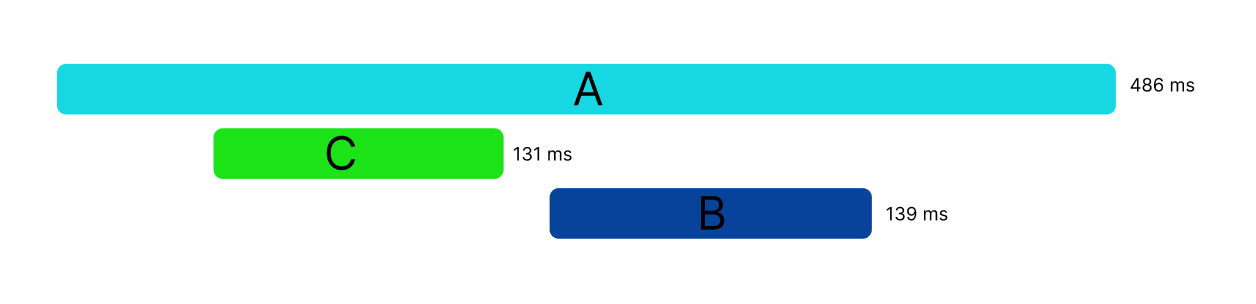
\includegraphics[width=15cm]{obrazky-figures/distributed_trace.png}
  \caption{Ukázka distribuované stopy}
  \label{fig:trace}
\end{figure}
Na obrázku \ref{fig:trace} vidíme jednu hlavní operaci s~názvem A, která obsahuje dvě podoperace B a C. Když nám monitorovací nástroj spojí operace dohromady, tak je nazýváme distribuované stopy.

  \subsubsection{Monitorovací data o~operaci (Span) }
  Operace reprezentují hlavní jednotku práce ve stopě. Operace v~systému OpenTelemetry se skládá z~následujících položek:
  \begin{itemize}
  \item{jména}
  \item{rodičovského ID operace – pro kořen je prázdný}
  \item{začáteční a koncový čas}
  \item{kontextu}
  \item{atributů}
  \item{událostí}
  \item{spojení}
  \item{statutu}
\end{itemize}
Na výpisu \ref{lst:spanJson} se můžeme podívat na ukázkové monitorovací data operace.

\begin{listing}[H]
    \begin{minted}{python}
{
  # identifikátor stopy, které operace náleží 
  "trace_id": "7bba9f33312b3dbb8b2c2c62bb7abe2d",
  "parent_id": "",
  # identifikátor operace 
  "span_id": "086e83747d0e381e",
  # název operace, který v~tomto případě nese cestu koncového bodu 
  "name": "/v1/sys/health",
  "start_time": "2021-10-22 16:04:01.209458162 +0000 UTC",
  "end_time": "2021-10-22 16:04:01.209514132 +0000 UTC",
  "status_code": "STATUS_CODE_OK",
  # atributy operace 
  "attributes": {
    "net.transport": "IP.TCP", # využitý protokol pro přenos 
    "net.peer.ip": "172.17.0.1", # vzdálená IP adresa 
    "net.peer.port": "51820", # vzdálený port 
    "net.host.ip": "10.177.2.152", # lokální IP adresa 
    "net.host.port": "26040", # lokální port 
    "http.method": "GET", # HTTP metoda požadavku 
    "http.target": "/v1/sys/health", /* cesta koncového bodu 
    "http.scheme": "http"  # využitý protokol 
  },
  # pole událostí operace 
  "events": [
    {
      "message": "OK",
      "timestamp": "2021-10-22 16:04:01.209512872 +0000 UTC"
    }
  ]
}
\end{minted}
    \caption{Ukázka operace ve formátu JSON představující HTTP GET požadavek}
    \label{lst:spanJson}
\end{listing}


Operace mohou být vnořené pomocí rodičovského ID operace. Tím dosáhneme lepšího porozumění toho, co se děje při provádění operace, která podoperace nás nejvíce zdržuje a co se během ní děje. Dále si popíšeme jednotlivé parametry operací a jejich význam.
    \begin{itemize}
    \item{\textbf{Kontext}}
    \item[]
    Kontext je neměnný soubor dat pro danou operaci a skládá se z~ID stopy, které náleží, unikátního klíče operace, příznaků stopy a stavu stopy. Stav je seznam atributů ve tvaru klíč-hodnota, jež nesou specifické informace pro daný nástroj.
    \item{\textbf{Atributy}}
    \item[]
    Atributy nesou data ve formátu klíč-hodnota, které obsahují metadata, pomocí nichž můžeme charakterizovat reálnou operaci, kterou mají monitorovací data představovat.

    Atribut musí splňovat následující pravidla platící pro každý programovací jazyk. Klíč musí být nenulový řetězec a hodnota může nabývat pouze nenulový řetězec, logickou hodnotou, desetinné číslo, celé číslo nebo pole těchto hodnot.
    \item{\textbf{Události}}
    \item[]
    Události si můžeme představit jako strukturovanou zprávu operace, jež má poukázat na významný okamžik v~průběhu operace. Pro lepší pochopení si to vysvětlíme na příkladu. Sledujeme načítaní dat ze serveru, takže vhodnou událostí by bylo, od kdy data byla dostupná.
    \item{\textbf{Spojení}}
    \item[]
    Spojení představuje propojení jedné operace s~další nebo více operacemi. Řekněme, že máme distribuovaný systém, v~němž sledujeme jeho operace pomocí stop.

    Při provedení některé z~operací se může jiná operace ocitnout ve frontě, kde čeká na provedení, jejíž provedení je však asynchronní. Obě operace sledujeme pomocí stop. Rádi bychom spojili stopu operace z~fronty s~hlavní operací, ale nemůžeme předvídat, kdy se operace spustí. Proto použijeme spojení na jejich propojení. Provedeme to tím, že poslední operace z~první stopy propojíme s~první operací z~druhé stopy.
    \item{\textbf{Status}}
    \item[]
    K~operaci přidáváme status pouze tehdy, když v~aplikaci nastane známá chyba, například výjimka. Může obsahovat jedno z~následujících označení:
    \begin{itemize}
        \item{Unset}
        \item{Ok}
        \item{Error}
    \end{itemize}
    Když výjimku zpracujeme, může být stav operace nastaven na \texttt{Error}. V~opačném případě je status nastaven na \texttt{Unset}. Nastavením stavu na \texttt{Unset} může monitorovací nástroj, který zpracovává telemetrická data operace, přiřadit konečný stav.
    \end{itemize}

\subsection{Metriky}
Metrická data \cite{Metrics} měříme a zachytáváme za běhu služby. Okamžik, kdy dojde k~zachycení dat, nazýváme metrická událost. Metrika se neskládá pouze z~dat měření, ale obsahuje i čas, kdy bylo měření provedeno a související metadata.

Jsou důležitým ukazatelem dostupnosti a vytíženosti aplikací a požadavků na rozhraní. Definováním vlastních metrických dat můžeme zjistit, jak dostupnost naší aplikace ovlivňuje například její návštěvnost. Nasbíraná data nás mohou upozornit na výpadek služby nebo můžeme podle nastavených pravidel automaticky škálovat aplikaci podle poptávky.

Systém OpenTelemetry definuje tři nástroje pro práci s~metrickými daty:
    \begin{itemize}
        \item{\textbf{Počítadlo (Counter)}}
        \item[]
        Počítadlo představuje hodnotu, která se v~čase sčítá a roste pouze nahoru. Můžeme si jej představit jako počet zápisů na disk.
        \item{\textbf{Součet (Measure)}}
        \item[]
        Součet slouží pro sčítání hodnot v~čase a je definovaný v~určitém rozsahu. Můžeme si ho představit jako počet ujetých kilometrů na tachometru.
        \item{\textbf{Pozorovatel (Observer)}}
        \item[]
        Pozorovatel zachycuje aktuální hodnoty v~určitou časovou dobu, například aktuální rychlost auta.
    \end{itemize}

    Dalším důležitým pojmem, se kterým se setkáváme u~metrických dat je agregace. Agregace je metoda, při které vezmeme velký počet naměřených vzorků a spojíme je do přesných nebo odhadovaných statistik o~metrických událostech, jež se odehráli v~určitém časovém rozmezí. Systém OpenTelemetry nám neumožňuje tyto agregace vytvářet, ale poskytuje nám běžně agregace, které podporují monitorovací nástroje a vizualizéry jako je suma, počet, poslední hodnota a histogramy.

    Metriky jsou určeny k~poskytování souhrnných statistických dat. Zde si ukážeme na co jsou vhodné:
    \begin{itemize}
        \item{využití procesoru nebo paměti}
        \item{počet požadavků na rozhraní}
        \item{měření latence operací}
        \item{hlášení aktuálně aktivních zpracovávaných požadavků}
    \end{itemize}
\subsection{Záznamy (Logs)}
Z~uvedených telemetrických dat jsou záznamy \cite{Logs} pravděpodobně nejznámějším a nejstarším způsobem sběru dat ze služeb nebo aplikací. Většina programovacích jazyků má podporu sběru záznamů již v~sobě zabudovanou nebo existuje knihovna pro daný jazyk. V~čem spočívá výhoda sběru záznamu v~systému OpenTelemetry si popíšeme později v~této kapitole.

Záznam uchováváme v~podobě textového zápisu s~časem, kdy byl záznam zachycen. Může být strukturovaný, což je doporučeno i v~dokumentaci, nebo v~nestrukturované podobě s~metadaty. Záznamy můžeme uchovávat samostatně, jako nezávislý zdroj dat, ale mohou být součástí operace. V~systému OpenTelemtry považujeme všechna data za záznamy, pokud nejsou obsažena v~distribuované stopě nebo metrice. Záznamy se často používají při pádu aplikace. Právě v~nich hledáme hlavní příčinu pádu a při jaké změně k~pádu došlo, ale to je jen jedna ukázka použití záznamu. Existuje jich mnoho typů, jako například:
    \begin{itemize}
        \item{\textbf{Záznam z~aplikace}}
        \item[]
        Záznam z~aplikace nese informaci o~události, jež se vyskytla za běhu aplikace.
        \item{\textbf{Systémové záznamy}}
        \item[]
        Systémové záznamy obsahují informaci o~samotném operačním systému, kde služba nebo aplikace běží.
        \item{\textbf{Síťové záznamy}}
        \item[]
        Síťové záznamy nám poskytují informace o~zařízeních v~infrastruktuře na základě aktivity v~síti.
        \item{\textbf{Záznamy z~webových serverů}}
        \item[]
        Záznamy z~webových serverů, jako je například Apache\footnote{Webový server Apache \url{https://apache.org/} [25.11.2022]}, lze použít pro identifikaci úzkých míst výkonu.
    \end{itemize}

\begin{figure}[h]
  \centering
  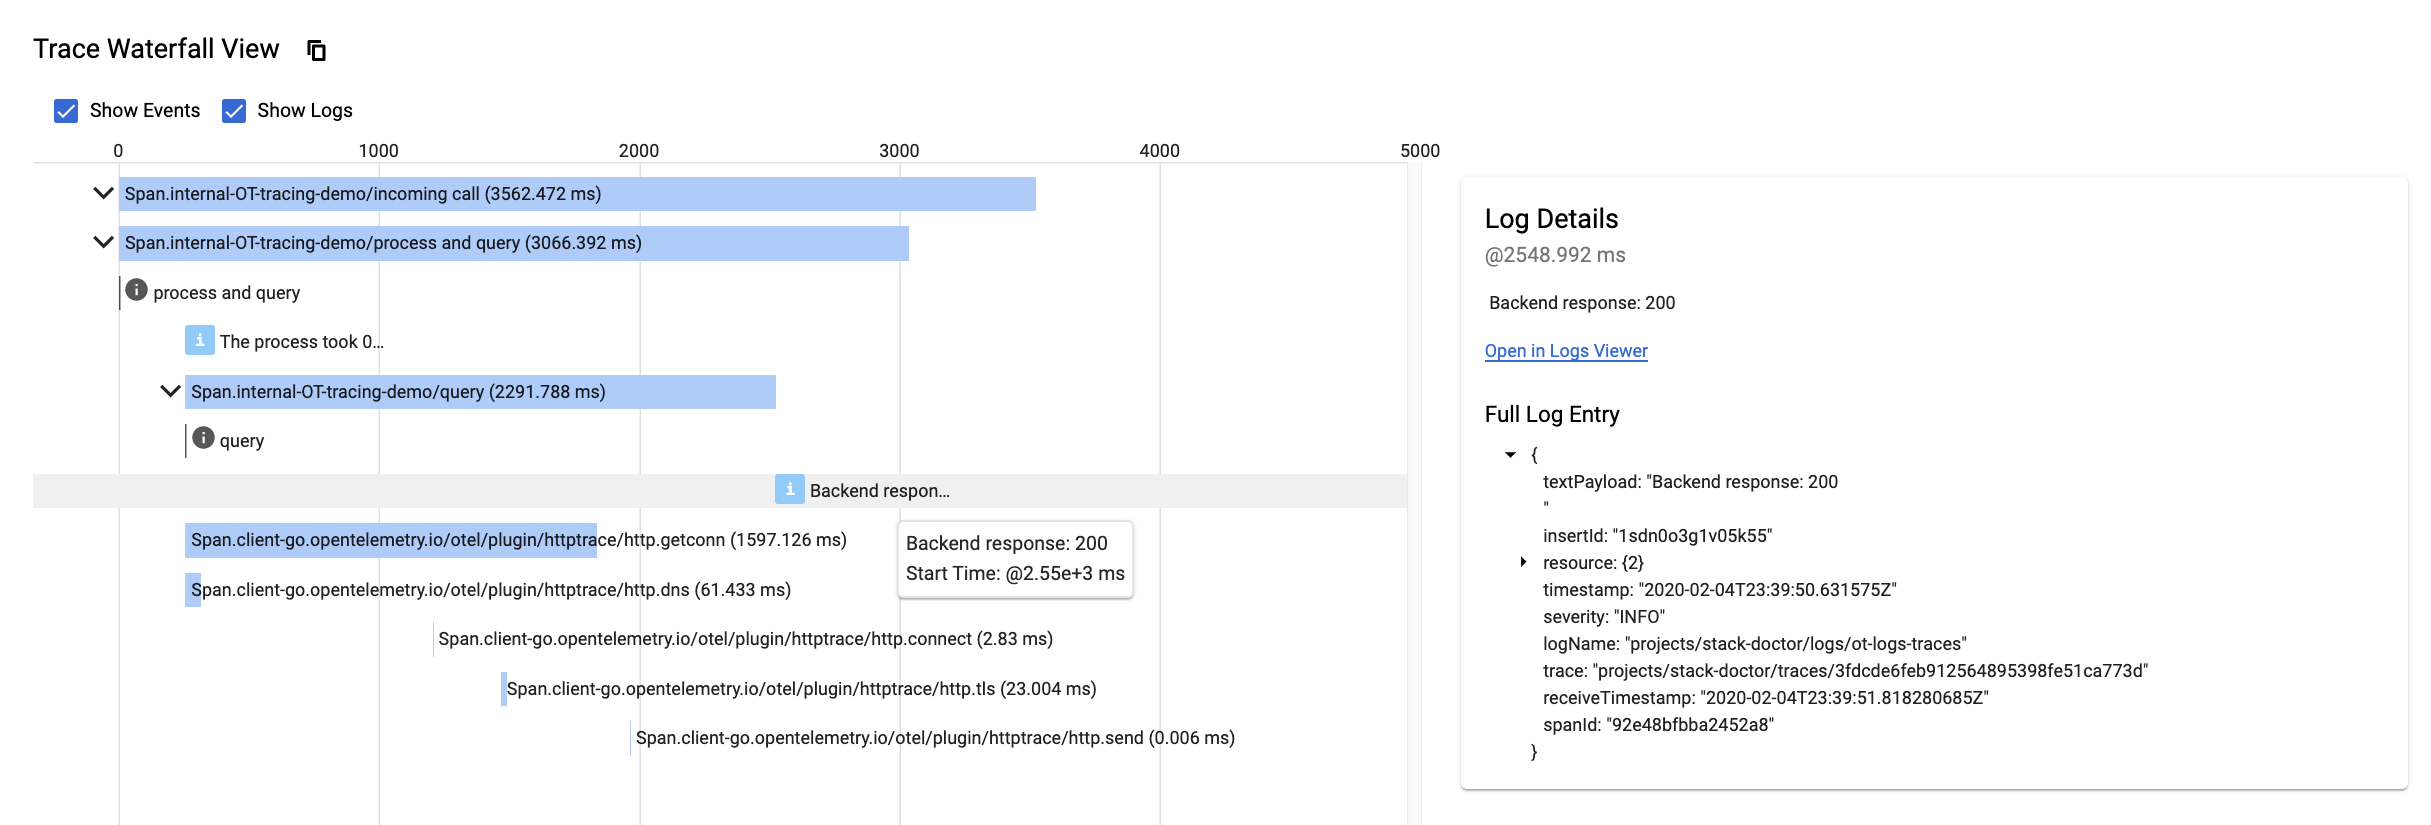
\includegraphics[width=15cm]{obrazky-figures/logSpan.png}
  \caption{Záznam připojený k~operaci\protect\footnotemark}
  \label{fig:log}
\end{figure}

\footnotetext{Obrázek byl převzat z~webu \url{https://medium.com/google-cloud/integrating-tracing-and-logging-with-opentelemetry-and-stackdriver-a5396fbc3e78} [25.11.2022]}

Na obrázku vidíme záznam, který nese textovou informaci v~podobě úspěšné odpovědi ze serveru, časovou značku kdy byl vytvořen a přijat monitorovacím nástrojem, název záznamu, identifikátor stopy a operace, které náleží.

\subsubsection{Výhody sběru záznamu se systémem OpenTelemetry}
Velké monitorovací nástroje by měly snadno umožňovat propojení telemetrických dat. Většina uživatelů, jež se snaží sbírat telemetrická data, používá pro každý telemetrický signál jiný nástroj a nemá možnost tyto signály propojit. Aktuální řešení sběru záznamu nepodporují propojení s~ostatními signály. Cílem systému OpenTelemetry je shromažďovat záznamy s~kontextem, aby mohly být později propojeny s~dalšími telemetrickými signály. \cite{SignozLog}

\subsubsection{Struktura záznamu/události systému OpenTelemetry}

Systém OpenTelemetry nedělá rozdíl mezi záznamem a událostí z~pohledu struktury dat. Pro obojí se využívá stejná struktura. Rozlišujeme je podle dat, která představují. Chceme-li zaznamenat pouze událost v~určitý čas, hovoříme o~události (výjimka v~kódu). Pokud potřebujeme zaznamenat další dodatečné informace o~události, poté mluvíme o~záznamem.


Struktura záznamu/události \cite{LogModel} byla navržen tak, aby umožňoval reprezentovat záznamy z~různých zdrojů. Díky tomu lze mapovat většinu záznamů třetích stran na strukturu záznamu systému OpenTelemetry. 

\begin{table}[H]
\centering
\begin{tabular}{|p{4cm}|p{4.3cm}|p{5.5cm}|}
\hline
\textbf{Název} & \textbf{Formát} & \textbf{Popis} \\ \hline
Časové razítko & uint64 & Čas, kdy událost nastala. \\ \hline
Časové razítko záznamu & uint64 & Čas, kdy byla událost zaznamenána. \\ \hline
ID stopy & sekvence bajtů & Identifikátor stopy \\ \hline
ID operace & sekvence bajtů & Identifikátor operace \\ \hline
Příznak stopy & byte & W3C příznak stopy \\ \hline
Text závažnosti & řetězec & Známe také jako úroveň záznamu \\ \hline
Číslo závažnosti & number & Číselná hodnota úrovně závažnosti \\ \hline
Tělo & řetězec & Tělo záznamu/události \\ \hline
Zdroj & map<řetězec, hodnota> & Popis zdroje záznamu/události \\ \hline
Místo generování & tuple s~řetězci & Místo odkud byl záznam vygenerován \\ \hline
Atributy & map<řetězec, hodnota> & Dodatečné informace o~záznamu/události \\ \hline
\end{tabular}
\caption{Struktura záznamu/události systému OpenTelemetry}
\end{table}


\begin{itemize}
        \item{\textbf{Časové razítko (Timestamp)}}
        \item[] 
            Čas je udaný v~nanosekundách od počátku unixového času. Hodnota je zaznamenána v~době, kdy událost nastala, a používá se čas zdroje. Pole je nepovinné.
        \item{\textbf{Časové razítko záznamu (ObservedTimestamp)}}
        \item[]
            Čas je udaný v~nanosekundách od počátku unixového času. Hodnota je zaznamenána při generování záznamu/události systémem OpenTelemetry, potom se toto pole rovná \texttt{Timestamp}. Pokud se jedná o~záznam, který pochází od třetí strany, tak se jedná o~čas, kdy systém OpenTelemetry (kolektor) přijal daný záznam. Pole je povinné.
        \item{\textbf{Pole pro kontext stopy}}
        \item[]
        \begin{itemize}
            \item{\textbf{ID stopy (TraceId)}}
            \item[]
                Pole je nastaveno, pokud je záznam/událost součástí stopy. Pole je nepovinné.
            \item{\textbf{ID operace (SpanId)}}
            \item[]
                Pole je nastaveno, pokud je záznam/událost součástí operace. Pole je nepovinné.
            \item{\textbf{Příznak stopy (TraceFlags)}}
            \item[]
                Poje je definováno specifikací W3C\footnote{Odkaz na W3C specifikaci. \url{https://www.w3.org/TR/trace-context/##trace-flags} [14.03.2023]} a nyní podporuje akorát jeden příznak \texttt{SAMPLED}. Pole je nepovinné.
            
        \end{itemize}
        \item{\textbf{Pole závažnosti}}
        \item[]
        \begin{itemize}
            \item{\textbf{Text závažnosti (SeverityText)}}
        \item[]
            Jedná se o~původní textovou reprezentaci závažnosti. Známou taky jako úroveň závažnosti. Pole je nepovinné.
        \item{\textbf{Číslo závažnosti (SeverityNumber)}}
        \item[]
            Jedná se o~číselnou hodnotu, která je definovaná specifikací systému OpenTelemetry. Pole je nepovinné.
        \end{itemize}
        \item{\textbf{Tělo (Body)}}
        \item[]
            Hodnota je obsažena v~tělu záznamu/události, zpráva může být čitelná pro lidi nebo to mohou být strukturovaná data. Pole je nepovinné.
        \item{\textbf{Zdroj (Resource)}}
        \item[]
            Popisujeme zdroj záznamu/události. Můžeme zde popsat, jaká aplikace záznam vytvořila a na jakém stroji běží. Pole je nepovinné.
        \item{\textbf{Místo generování (InstrumentationScope)}}
        \item[]
            Popisujeme, z~jakého místa v~kódu byl záznam/událost vygenerován. Záznamy/události pocházející z~jednoho místa mají stejnou hodnotu. Pole je nepovinné.
        \item{\textbf{Atributy (Attributes)}}
        \item[]
        Jedná se o~dodatečné informace o~události, jež nastala. Například se hodnota může lišit, i když událost nastala ve stejné aplikaci. V~tom případě by nám nepomohlo pole \texttt{Zdroj}, ale mělo by nám pomoct pole \texttt{Atributy}. Můžeme zde uvádět informace například o~verzi knihoven, které aplikace aktuálně využívá.
    \end{itemize}

\begin{listing}[H]
    \begin{minted}{json}
{
  "Timestamp": 1586960586000,
  "TraceId": "f4dbb3edd765f620",
  "SpanId": "43222c2d51a7abe3",
  "SeverityText": "INFO",
  "SeverityNumber": 9,
  "Body": "20200415T072306-0700 INFO I~like donuts",
  "Resource": {
    "service.name": "donut_shop",
    "service.version": "semver:2.0.0",
    "k8s.pod.uid": "1138528c-c36e-11e9-a1a7-42010a800198",
  },
  "Attributes": {
    "http.status_code": 500,
    "http.url": "http://example.com",
    "my.custom.application.tag": "hello",
  }
}
\end{minted}
    \caption{Ukázka záznamu v~JSON formátu}
    \label{lst:exampleLog}
\end{listing}

\subsection{Sdílená data stopy (Baggage)}

V~systému OpenTelemetry signálem \textit{Baggage} \cite{Baggage} označujeme informace, které se předávají mezi jednotlivými operacemi. Můžeme si je představit jako úložiště, jež obsahuje data ve formě klíč-hodnota. K~těmto datům mají přístup pouze operace z~jedné stopy. V~systému OpenTelemetry pro předávání dat se používá již vysvětlená kontextová propagace. Například jako klíč použijeme text \texttt{id\textunderscore osoby} a jako hodnotu unikátní klíč dané osoby \texttt{0108204256} v~tomto případě rodné číslo.


\begin{figure}[H]
  \centering
  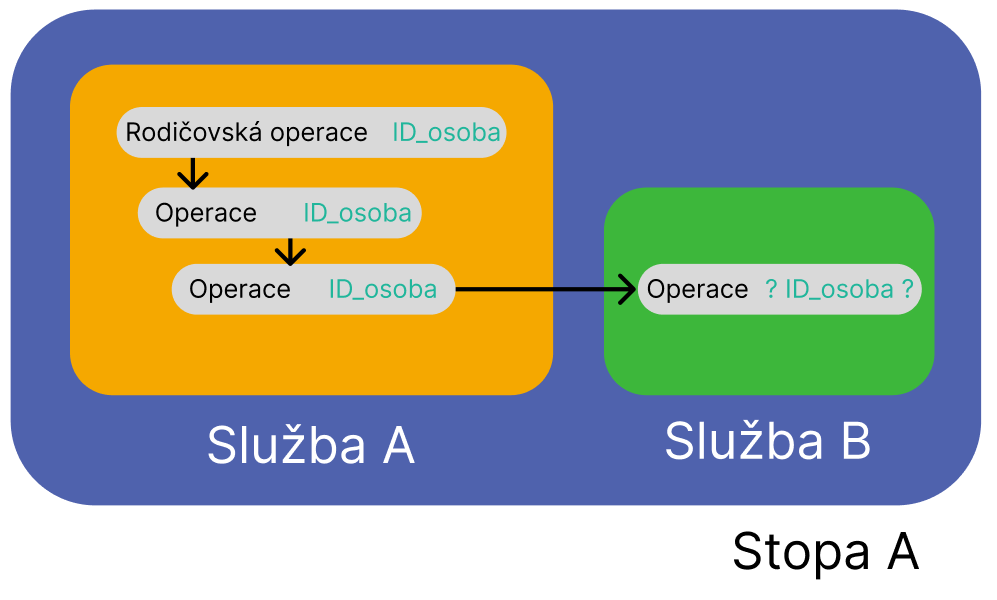
\includegraphics[width=14cm]{obrazky-figures/baggage.png}
  \caption{Stopa s~neznámým ID\textunderscore osoby ve službě B}
  \label{fig:baggage}
\end{figure}


Na obrázku \ref{fig:baggage} vidíme jednu stopu pojmenovanou A. Představme si, že znázorňuje nákup lístků do kina, kde služba A~představuje přidání lístku do košíku a služba B kontrolu počtu volných lístků. V~jednotlivých operacích si zaznamenáváme, která osoba danou podoperaci provedla. V~momentě kdy služba A~zavolá službu B a chceme si poznamenat v~operaci služby B Id osoby, která danou akci provedla, tak služba B nemá přístup k~této informaci. V~tom případě musíme využít sdílená data. Na začátku si tam uložíme Id osoby a poté ho můžeme kdykoliv ve stopě A~přečíst a zapsat jej, kde potřebujeme.

\subsubsection{Proč používat sdílená data}
Jelikož systém OpenTelemetry je nezávislý na platformě a použitém programovacím jazyku, tak díky sdílení dat docílíme toho, že můžeme analyzovat, číst a používat data ve všech aplikacích bez ohledu na to, ve kterém programovacím jazyce byly napsány.

To je důležité, když vytváříme velký monitorovací systém, kde jsou aplikace napsány v~různých programovacích jazycích. Tím poskytujeme vývojářům aplikací volnou ruku při výběru technologie pro vývoj.

Přidáváním dodatečných dat do signálů v~navazujících službách, nám zajistí lepší filtrování a vyhledávání v~monitorovacích nástrojích.

\subsubsection{Vhodné použití}

Ve sdílených datech by se měla uchovávat jen necitlivá data, protože mohou být vystavena třetím stranám. Vhodná data jsou například:
\begin{itemize}
        \item{identifikátor osoby}
        \item{IP adresa odesílatele}
        \item{verze webového serveru}
\end{itemize}


\section{Sběr telemetrických dat}

Systém OpenTelemetry nám umožňuje sbírat telemetrická data dvěma způsoby. Podporuje manuální a automatický sběr nebo můžeme kombinovat oba způsoby tím, že použijeme automatický sběr a manuálně přidáváme informace do existujících dat nebo vytváříme úplně nová. V~následujících dvou podkapitolách si popíšeme jednotlivé způsoby podrobněji a ukážeme si názornou ukázku v~jazyce Python.

\subsection{Automatický sběr dat}
Využitím automatického sběru dat nám odpadá povinnost psát kód pro každou operaci v~aplikaci. Stačí nám nainstalovat knihovnu \texttt{opentelemetry-distro}, která nám zařídí sběr telemetrických dat. Musíme také nastavit, kam budeme telemetrická data odesílat a to pomocí parametru při spouštění programu. Ukázku si můžeme prohlédnout v~příloze \ref{auto}.
\begin{listing}[H]
    \begin{minted}{python}
        opentelemetry-instrument --traces_exporter console python app.py
    \end{minted}
    \caption{Příkaz pro spuštění programu app s~výpisem stop do příkazové řádky}
    \label{lst:bash1}
\end{listing}


Nebo můžeme místo nastavit pomocí \textit{environment variables}, kde nastavíme hodnoty \newline \texttt{OTEL\textunderscore TRACES\textunderscore EXPORTER} a \texttt{OTEL\textunderscore METRICS\textunderscore EXPORTER}.
\begin{listing}[H]
    \begin{minted}{python}
        opentelemetry-instrument python app.py
    \end{minted}
    \caption{Příkaz pro spuštění programu app}
    \label{lst:bash2}
\end{listing}

\subsection{Manuální sběr dat}

Při manuálním sběru dat musíme přidat kód do aplikace pro jednotlivé operace, jež chceme pozorovat. Bohužel si ukážeme pouze stopy a metriky, protože záznamy jsou u~programovacích jazyků ve vývoji nebo je zatím nepodporují vůbec. Ukázku si můžeme prohlédnout v~příloze \ref{manual}.
    
V~následujících ukázkách potřebujeme knihovny \texttt{opentelemetry-api} a \\ \texttt{opentelemetry-sdk}, které budeme vyžívat k~manuálnímu sběru dat.

\subsubsection{Sběr stop}
Na začátku musíme inicializovat \texttt{TracerProvider}, pomocí kterého vytváříme distribuované stopy a operace. Ve výpisu \ref{lst:exampleTraceProvider} vidíme také ještě výpis dat do příkazové řádky pomocí metody \texttt{ConsoleSpanExporter}.

\begin{listing}[H]
    \begin{minted}{python}
from opentelemetry import trace
from opentelemetry.sdk.trace import TracerProvider
from opentelemetry.sdk.trace.export import (
    BatchSpanProcessor,
    ConsoleSpanExporter,
)

provider = TracerProvider()
processor = BatchSpanProcessor(ConsoleSpanExporter())
provider.add_span_processor(processor)

# Nastavení globálního TraceProvideru
trace.set_tracer_provider(provider)

# Inicializace proměnné tracer pomocí, které budeme  
# vytvářet jednotlivé operace
tracer = trace.get_tracer(__name__)
\end{minted}
    \caption{Základní inicializace pro sběr stop}
    \label{lst:exampleTraceProvider}
\end{listing}

Ve výpisu \ref{lst:exampleTraces} vidíme vytvoření distribuované stopy, která se skládá ze dvou operací. Jedné hlavní, která obsahuje vnořenou operaci.

\begin{listing}[H]
    \begin{minted}{python}
def square():
    with tracer.start_as_current_span("parent") as parent:
        # rodičovská operace
        number = random()
        # Vytvoření vnořené operace
        with tracer.start_as_current_span("child") as child:
            return number * number
\end{minted}
    \caption{Vytvoření distribuované stopy}
    \label{lst:exampleTraces}
\end{listing}

Získání aktuální operace můžeme využít i při automatickém sběru dat a doplnit dodatečné informace k~operaci. Získání aktuální operace, kterou budeme používat v~dalších ukázkách pro přidávání dodatečných informací do operace vidíme ve výpisu \ref{lst:exampleCurrentTraces}.
\begin{listing}[H]
    \begin{minted}{python}
from opentelemetry import trace

current_span = trace.get_current_span()
\end{minted}
    \caption{Získání aktuální operace}
    \label{lst:exampleCurrentTraces}
\end{listing}
Ve výpisu \ref{lst:exampleTraceAtribute} vidíme přidání vlastního atributu do operace nebo využití předdefinovaného jména atributu. Pro využití předem nadefinovaných jmen atributů musíme nainstalovat balíček \texttt{opentelemetry-semantic-conventions}.

\begin{listing}[H]
    \begin{minted}{python}
from opentelemetry.semconv.trace import SpanAttributes
    
# Vlastní atribut    
current_span.set_attribute("some.value", 1)

# Předdefinovaný název atributu
current_span.set_attribute(SpanAttributes.HTTP_METHOD, "GET")
\end{minted}
    \caption{Přidání atributu do operace}
    \label{lst:exampleTraceAtribute}
\end{listing}

Ve výpisu \ref{lst:exampleTraceEvent} vidíme přidání události operace, která obsahuje zprávu čitelnou pro člověka.

\begin{listing}[H]
    \begin{minted}{python}
current_span.add_event("Some interesting message!")
\end{minted}
    \caption{Přidání události do operace}
    \label{lst:exampleTraceEvent}
\end{listing}

Operace mohou mít žádné nebo více spojení. V~tomto případě nemyslíme vnořené operace. Ve výpisu \ref{lst:exampleTraceLink} vidíme kde pomocí kontextu jedné operace vytvoříme novou a tím definujeme spojení mezi nimi.

\begin{listing}[H]
    \begin{minted}{python}
contex = trace.get_current_span().get_span_context()

link = trace.Link(contex)

with tracer.start_as_current_span("new-span", links=[link]) as new_span:
    # Kód pro operaci, kterou zaznamenáváme
\end{minted}
    \caption{Vytvoření spojení mezi dvěma operacemi}
    \label{lst:exampleTraceLink}
\end{listing}

Pokud chceme ukládat v~operaci informaci o~návratovém kódu nebo chceme uložit zachycenou výjimku a její zprávu, využíváme k~tomu statusu. Ve výpisu \ref{lst:exampleTraceStatus} vidíme uložení informace o~výjimce a nastavení statusu.

\begin{listing}[H]
    \begin{minted}{python}
from opentelemetry.trace import Status, StatusCode
    
try:
    # Kód, který může selhat
except Exception as ex:
    current_span.set_status(Status(StatusCode.ERROR))
    current_span.record_exception(ex)
\end{minted}
    \caption{Zaznamenání statutu a výjimky v~operaci}
    \label{lst:exampleTraceStatus}
\end{listing}



\subsubsection{Sběr metrik}

Na začátku musíme inicializovat \texttt{MeterProvider}, pomocí kterého vytváříme metriky a nastavit kam budeme data odesílat. Ve výpisu \ref{lst:exampleMeterProvider} vidíme také ještě výpis dat do příkazové řádky pomocí metody \texttt{ConsoleMetricExporter}.

\begin{listing}[H]
    \begin{minted}{python}
from opentelemetry import metrics
from opentelemetry.sdk.metrics import MeterProvider
from opentelemetry.sdk.metrics.export import (
    ConsoleMetricExporter,
    PeriodicExportingMetricReader,
)

metric_reader = PeriodicExportingMetricReader(ConsoleMetricExporter())
provider = MeterProvider(metric_readers=[metric_reader])

# Nastavení globálního MeterProvideru
metrics.set_meter_provider(provider)

# Inicializace proměnné meter pomocí,
# které poté budeme vytvářet jednotlivé metriky
meter = metrics.get_meter(__name__)
\end{minted}
    \caption{Základní inicializace pro sběr metrik}
    \label{lst:exampleMeterProvider}
\end{listing}

Nejprve si inicializujeme globální metriku, která se vytváří pouze jednou a poté voláme pouze metody podle dané metriky. Ve výpisu \ref{lst:exampleMetrics} si ukážeme počítadlo pro počet zavolání metody \texttt{square}.

\begin{listing}[H]
    \begin{minted}{python}
square_counter = meter.create_counter("square.counter", unit="1",
    description="Counts number calls of the method"
)

def square(number):
    # Zvýšíme počítadlo
    square_counter.add(1, {"square.number": number})
    return number*number
\end{minted}
    \caption{Základní inicializace pro sběr metrik}
    \label{lst:exampleMetrics}
\end{listing}

\section{Architektura}
\label{architektura}
V~systému OpenTelemetry se architektura skládá z~několika hlavních komponentů, jež umožňují sběr, úpravu a odesílání telemetrických dat. Hlavní komponentou je kolektor (Collector), který přijímá data od všech poskytovatelů a odesílá je na monitorovací nástroje.

\begin{figure}[H]
  \centering
  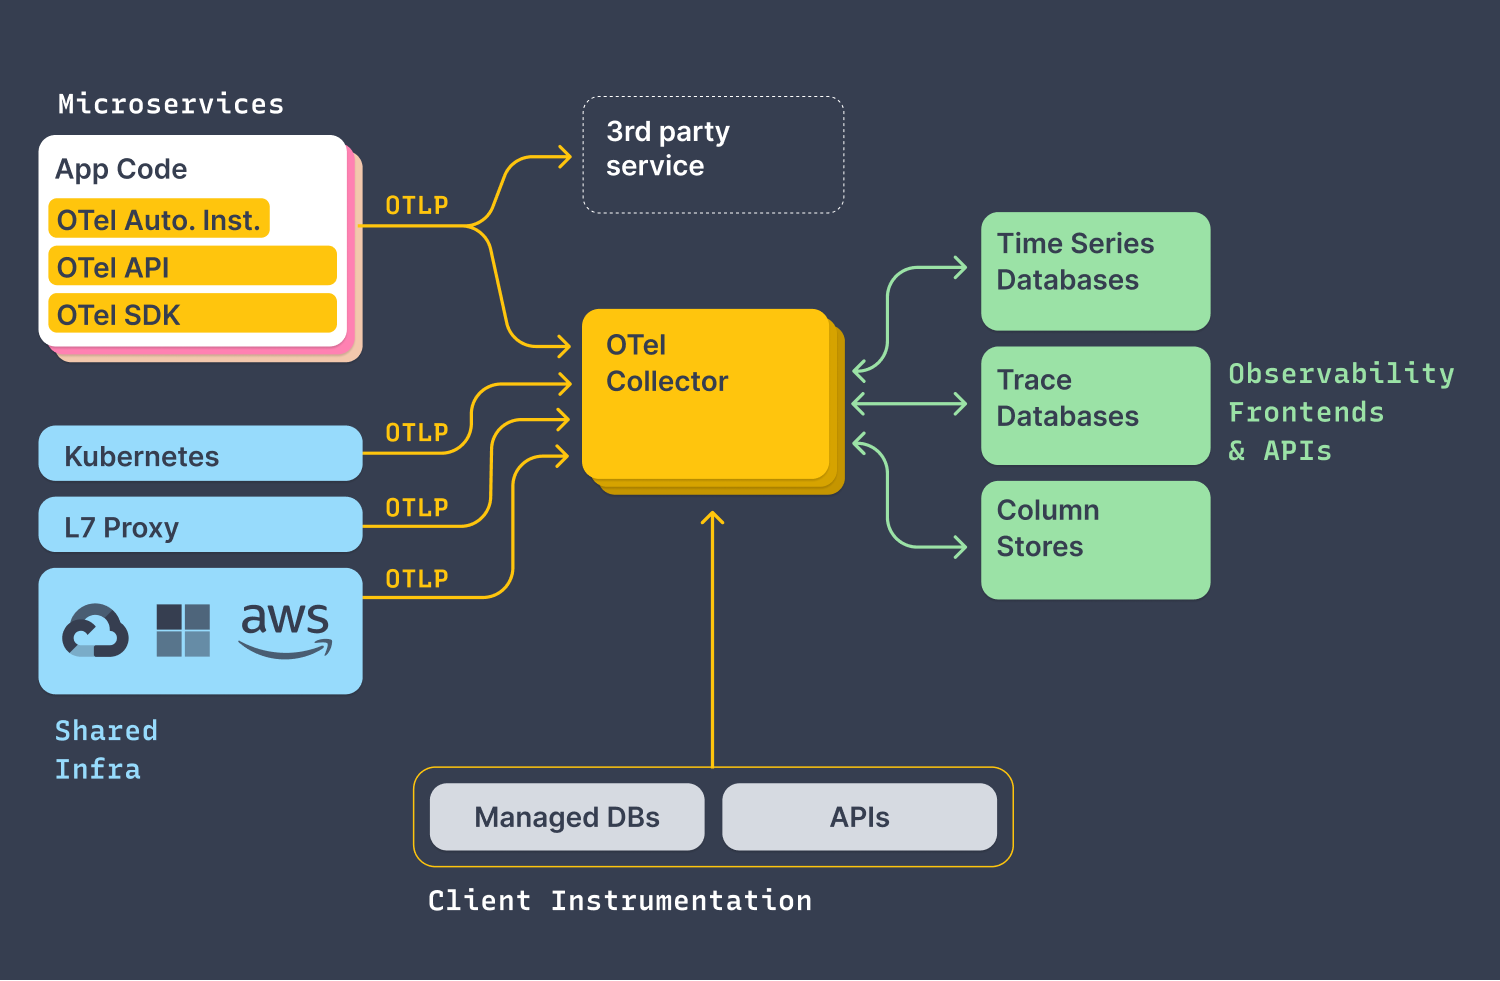
\includegraphics[width=12cm]{obrazky-figures/otel_diagram.png}
  \caption{Doporučená architektura\protect\footnotemark}
  \label{fig:architecture}
\end{figure}
\footnotetext{Obrázek byl převzat z~webu \url{https://opentelemetry.io/docs/} [29.11.2022]}

Na obrázku \ref{fig:architecture} vidíme architekturu, kde se uprostřed nachází kolektor (OTel Collector), který přijímá telemetrické signály pomocí OpenTelemetry protokolu (OTLP). Můžeme si povšimnout, že data nemusíme přijímat jen lokálně, kde máme nasazený kolektor, ale dokážeme data přijímat od poskytovatelů cloudových služeb, jako je například AWS\footnote{Amazon Web Services – poskytovatel cloudových služeb \url{https://aws.amazon.com/} [29.11.2022]}, Azure\footnote{Microsoft Azure – cloudové výpočetní služby  \url{https://azure.microsoft.com/en-us/} [29.11.2022]} a mnoho dalších. Kolektor nadále data zpracuje a odesílá je do aplikace, kde jsou uživateli data zobrazeny a současně je ukládá do databáze.
    
\subsection{Kolektor (Collector)}

Kolektor \cite{SignozCollector} nabízí způsob přijímaní, zpracování a odesílaní dat nezávisle na dodavateli. Tudíž odstraňuje potřebu mít vlastní sběrač dat pro každý protokol nebo dokonce pro jednotlivá telemetrická data. Podporuje příjem telemetrických dat od mnoha dodavatelů s~otevřeným zdrojovým kódem, jako jsou například Jaeger, Fluent Bit, Prometheus a mnoho dalších. Telemetrická data po zpracování odesílá do jednoho nebo více monitorovacích nástrojů. Kolektor je výchozím místem, kam knihovny pro generovaní telemetrických dat odesílají svá data.
\begin{figure}[H]
  \centering
  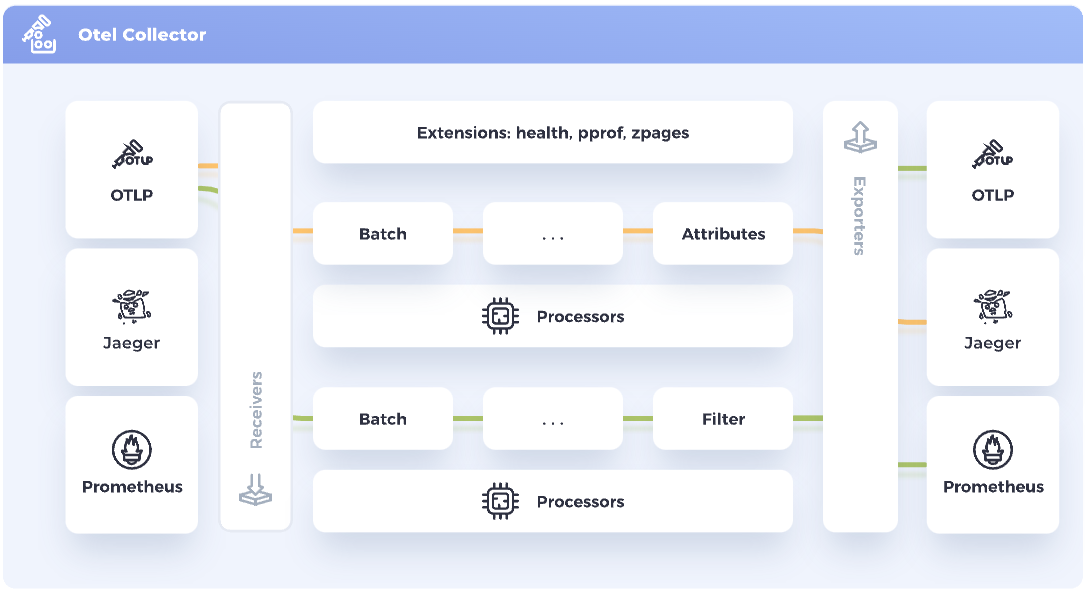
\includegraphics[width=14cm]{obrazky-figures/otel_collector.png}
  \caption{Ukázka architektury kolektoru\protect\footnotemark}
  \label{fig:collector}
\end{figure}
\footnotetext{Obrázek byl převzat z~webu \url{https://raw.githubusercontent.com/open-telemetry/opentelemetry.io/main/iconography/Otel_Collector.svg} [29.11.2022]}
Na obrázku \ref{fig:collector} vidíme architekturu kolektoru, která se skládá ze tří částí. První je přijímač (Receivers), který dokáže přijímat data v~různých formátech. V~tomto případě přijímá dvoje telemetrická data pomocí OpenTelemetry protokolu (OTLP), která jsou naznačena zelenou a žlutou trasou. Druhou částí je procesor, který může manipulovat s~odesílanými daty. Poslední částí je exportér (Exporters), který odesílá zpracovaná telemetrická data pomocí podporovaných protokolů do monitorovacích nástrojů. V~tomto případě odesílá data zelené trasy pomocí Prometheus a OpenTelemetry protokolu a žluté trasy Jaeger protokolem. Nyní se podíváme na jednotlivé komponenty kolektoru podrobněji.
    \begin{itemize}
        \item{\textbf{Přijímač (Receivers)}}
        \item[]
        Přijímačem vstupují data do kolektoru. Existují dva druhy. První naslouchá a čeká na služby, až mu odešlou telemetrická data a druhý, který si stahuje data ze služeb. Jak již bylo řečeno, dokáže přijímat data v~mnoha formátech. Ve výchozím stavu je přijímač nastaven na OpenTelemetry protokol. Po přijetí se data převedou do interního formátu kolektoru a jsou předána procesoru.
        \item{\textbf{Procesor (Processors)}}
        \item[]
        Procesor zpracovává nashromážděná telemetrická data před jejich předáním exportéru. Dokáže provést jakoukoliv úpravu dat při jejich průchodu. Pokud data mají být zveřejněna, můžeme odstranit osobní údaje uživatelů z~telemetrických dat. Podporuje také dávkování dat před odesláním, jejich znovu odeslání, pokud exportér selže, přidávaní metadat a mnoho dalšího.
        \item{\textbf{Exportér (Exporters)}}
        \item[]
        Exportér umožňuje odesílání zpracovaných dat do monitorovacích nástrojů. Můžeme odesílat jedny telemetrická data do více nástrojů nebo je rozdělit. Například odesílat stopy do monitorovacího nástroje a záznamy vypisovat na standardní výstup.
    \end{itemize}

Systém OpenTelemetry nám umožňuje odesílat data přímo do monitorovacích nástrojů. Tady nám vzniká otázka: „Proč bychom vlastně měli používat kolektor?“ Na tuto otázku si odpovíme následujícím výčtem výhod kolektoru.
    \begin{itemize}
        \item{nezávislý sběr telemetrických dat na protokolu}
        \item{přebírá odpovědnost za správu telemetrických dat od aplikace}
        \item{umožňuje exportovat data v~různých formátech do více monitorovacích nástrojů}
        \item{jednotná konfigurace sběru a odesílání telemetrických dat}
    \end{itemize}
    
\subsection{Rozhraní (API)}
Doposud jsme si popsali, jaká telemetrická data sbíráme, a jak vypadají, ale systém OpenTelemetry také definuje, jak s~telemetrickými daty pracovat.

OpenTelemetry API specifikuje a popisuje třídy a jejich funkce pro interakci s~telemetrickými daty. Například popisuje, jak systém OpenTelemetry může implementovat generování stop nebo hlásit metrická měření.

Specifikace API obsahuje dvě základní složky:
\begin{itemize}
        \item{definici rozhraní, které používáme pro práci s~telemetrickými daty,}
        \item{minimální implementaci tohoto rozhraní.}
    \end{itemize}

\subsection{Sada nástrojů pro generování telemetrických dat (SDK)}
Systém OpenTelemetry nabízí pro podporované programovací jazyky sadu nástrojů, které umožňují používat OpenTelemetry rozhraní ke generování telemetrických dat a exportovat je do kolektoru, nebo přímo do monitorovacího nástroje.

Každá sada nástrojů by minimálně měla obsahovat:
    \begin{itemize}
        \item{nezávislý sběr telemetrických dat na protokolu,}
        \item{přebírá odpovědnost za správu telemetrických dat od aplikace,}
        \item{umožňuje exportovat data v~různých formátech do více monitorovacích nástrojů.}
    \end{itemize}

\section{Protokol OTLP}
Systém OpenTelemetry definuje specifikaci protokolu OTLP (OpenTelemetry protokol) \cite{OTLP} pro přenos telemetrických dat bez ohledu na monitorovací nástroj a poskytovatele dat. Díky této vlastnosti je výměna monitorovacího nástroje snadná. 

Pomocí OTLP můžeme přenášet telemetrická data z~SDK do kolektoru a z~kolektoru do monitorovacího nástroje. Specifikace OTLP definuje kódování, transport a mechanismus doručování telemetrických dat.

\subsection{Detaily protokolu}
OpenTelemetry protokol definuje kódování telemetrických dat a protokol používaný k~výměně dat mezi klientem a serverem. Tato specifikace definuje jak OpenTelemetry protokol implementuje transport dat přes gRPC\footnote{Vzdálené volání procedur \url{https://grpc.io/} [4.12.2022]} a HTTP 1.1. Specifikuje také schéma pro serializaci dat pomocí Protocol Buffers\footnote{Mechanizmus pro serializaci strukturovaných dat \url{https://developers.google.com/protocol-buffers/docs/overview} [4.12.2022]}.

Komunikuje pomocí požadavku a odpovědi, kde klient pošle požadavek na server a dostane ze serveru odpověď.

Všechny servery, které chtějí používat OpenTelemetry protokol, musí podporovat tyto metody komprese:
\begin{itemize}
    \item{bez komprese,}
    \item{Gzip komprese.}
\end{itemize}
\subsection{Protokoly OTLP a gRPC}
Po navázání úvodního spojení gRPC, začne klient odesílat telemetrická data unárními požadavky\footnote{Unární komunikace je tradiční komunikace požadavek-odpověď používaný také v~protokolu HTTP.} pomocí tzv. \textit{ExportServiceRequest} zpráv. 
\begin{itemize}
        \item{Pro záznamy se nazývá \textit{ExportLogsServiceRequest}}
        \item{Pro stopy se nazývá \textit{ExportTraceServiceRequest}}
        \item{Pro metriky se nazývá \textit{ExportMetricsServiceRequest}}
\end{itemize}
Komunikace vždy probíhá jednou dvojicí klientem a serverem. Klient průběžně odesílá požadavky na server a čeká na potvrzení o~přijetí. Výchozí port je 4317.
\begin{figure}[H]
  \centering
  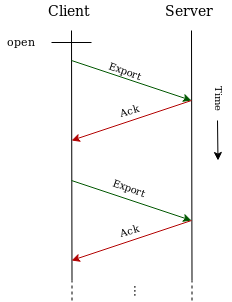
\includegraphics[width=4cm]{obrazky-figures/otlp-request-response.png}
  \caption{Ukázka unární komunikace mezi klientem a serverem\protect\footnotemark}
  \label{fig:oltp}
\end{figure}
\footnotetext{Obrázek byl převzat z~webu \url{https://opentelemetry.io/docs/reference/specification/protocol/img/otlp-request-response.png} [19.12.2022]}
Během požadavku mezi klientem a serverem, by nemělo dojít ke ztrátě dat. Záruka není garantována, pokud data putují přes více uzlů, jako například: aplikace > agent > kolektor > monitorovací nástroj.

\subsubsection{Sekvenční a souběžné požadavky}
Protokoly OTLP a gRPC podporují souběžné a sekvenční odesílání požadavků.

Sekvenční odesílaní znamená, kdy klient odešle jeden požadavek a čeká na potvrzení od serveru, než odešle další. Komunikace takhle pokračuje, než se spojení ukončí. Tento způsob komunikace se doporučuje, když vyžadujeme jednoduchou implementaci a server a klient se nachází v~síti s~malou latencí.
\begin{figure}[H]
  \centering
  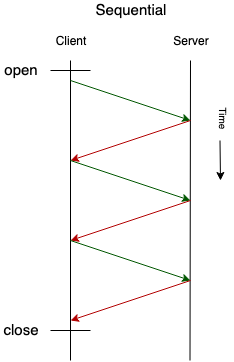
\includegraphics[width=4cm]{obrazky-figures/otlp-sequential.png}
  \caption{Ukázka sekvenční komunikace\protect\footnotemark}
  \label{fig:oltp-sequence}
\end{figure}
\footnotetext{Obrázek byl převzat z~webu \url{https://opentelemetry.io/docs/reference/specification/protocol/img/otlp-sequential.png} [19.12.2022]}

Souběžné odesílání používáme, když chceme dosáhnout velké propustnosti. Klient tedy nemusí čekat před odesláním nového požadavku, než mu přijde potvrzení na předchozí.

\begin{figure}[H]
  \centering
  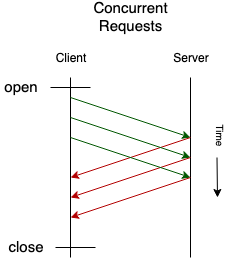
\includegraphics[width=4cm]{obrazky-figures/otlp-concurrent.png}
  \caption{Ukázka souběžných komunikace\protect\footnotemark}
  \label{fig:oltp-concurrent}
\end{figure}
\footnotetext{Obrázek byl převzat z~webu \url{https://opentelemetry.io/docs/reference/specification/protocol/img/otlp-concurrent.png} [19.12.2022]}

Spojení ukončujeme tím, že klient počká na všechna potvrzení od serveru nebo až vyprší časový limit, jež je specifický pro implementaci. Tím je zajištěno spolehlivé doručení telemetrických dat. Pokud klient není schopen doručit požadavek serveru, například při čekaní na potvrzení od serveru a vyprší u~toho časový limit. Klient by měl zaznamenat danou skutečnost, že data nebyla doručena.

\subsubsection{Odpověď ze serveru}
Odpověď je reakce serveru na klientův požadavek. Odpověď musí mít určitý formát, který si popíšeme v~následujících bodech.
    \begin{itemize}
        \item{\textbf{Úspěch (Full Success)}}
        \item[]
        Úspěšnou zprávu můžeme očekávat, pokud byla všechna telemetrická data přenesena nebo byl požadavek prázdný. V~obou případech odesíláme úspěšnou odpověď.
        \item{\textbf{Částečný úspěch (Partial Success)}}
        \item[]
        Částečný úspěch nastane, když server přijme jenom část telemetrických dat a zbytek odmítne. Ve zprávě inicializuje pole \textit{partial\textunderscore  success} a nastavíme \textit{rejected\textunderscore  spans}, \textit{rejected\textunderscore data\textunderscore points} a \textit{rejected\textunderscore log\textunderscore records} podle počtu odmítnutých stop, metrik a záznamů. Server podle chyby může vyplnit pole \textit{error\textunderscore  message} se zprávou čitelnou pro člověka, která popisuje chybu, jak ji může vyřešit a kde najít další informace.
        \item{\textbf{Selhání (Failure)}}
        \item[]
        Selhání dělíme na dvě kategorie: opravitelné a neopravitelné.
        \begin{itemize}
            \item{Opravitelné selhání znamená, když server není schopen zpracovat telemetrická data. Klient obdrží zprávu se selháním, ale s~informací, že může opakovat odeslaní dat. Server označí zprávu pomocí kódu \textit{Unavailable} a můžeme poskytnout další informace pomocí statusu \textit{RetryInfo}.}
            \item{Neopravitelné selhání znamená, když nastane chyba například při deserializaci špatných dat. Klient obdrží zprávu o~neopravitelném selhání, takže telemetrická data nesmí být odeslána znova. Klient musí daná data zahodit a zvýšit počítadlo, kde si uchovává kolik telemetrických dat zahodil. Server musí zprávu označit, aby klient poznal, že se jedná o~neopravitelnou chybu. Označí ji pomocí \textit{InvalidArgument} a další informace můžeme poskytnout pomocí statusu \textit{BadRequest}.}
        \end{itemize}
    \end{itemize}
\subsubsection{Zpomalení požadavků (Throttling)}
Protokol OpenTelemetry podporuje signalizaci přetížení. Pokud server není schopen přijímat tolik dat, musí danou situaci oznámit klientovi, aby se zabránilo přetížení serveru. Server oznámí tuto událost pomocí chyby s~kódem \textit{Unavailable}.

\subsection{Protokoly OTLP a HTTP}
Protokol používá Protobuf kódování pro přenos telemetrických dat v~binární formě nebo ve formátu JSON. Výchozí port je 4318. 

Pro přenos telemetrických dat využívá POST požadavků z~klienta na server. Můžeme využívat protokol HTTP/1.1 nebo HTTP/2, ale vždy daná implementace musí podporovat HTTP/1.1, kdyby došlo k~selhání HTTP/2.

\subsubsection{Kódování binárních dat pomocí Protobuf}
Telemetrická data v~binární podobě jsou zakódovaná pomocí standardu proto3\footnote{Specifikace standardu \url{https://developers.google.com/protocol-buffers/docs/proto3}}. Aby klient a server věděl, že dané kódování využíváme, musíme mít nastaveno v~HTTP hlavičce \texttt{Content-Type: application/x-protobuf} u~požadavku i odpovědi.

\subsubsection{Kódování dat ve formátu JSON pomocí Protobuf}
Využívá se stejný standard jako u~dat v~binární podobě a využívá se tzv. JSON mapovaní mezi Protobuf formátem a JSON formátem, ale pro potřeby OpenTelemetry protokolu je zde pár odchylek:
\begin{itemize}
        \item{hodnoty \texttt{trace\textunderscore id} a \texttt{span\textunderscore id} jsou reprezentovány pomocí řetězce bez rozlišení velkých a malých písmen v~base16\protect\footnotemark,}
        \item{výčtové typy (enum) mohou být převedeny pouze jako celé číslo,}
        \item{klíče v~JSON objektu jsou převáděny na tzv. camel case.}
\end{itemize}
\footnotetext{Specifikace base16 \url{https://www.rfc-editor.org/rfc/rfc4648\#section-8} [21.12.2022]}

Stejně jako u~binárních dat musí být u~klienta i serveru nastaven u~požadavků a odpovědí \texttt{Content-Type: application/x-protobuf}.

\subsubsection{HTTP požadavky}
Telemetrická data posíláme pomocí HTTP POST požadavků. Jsou nadefinované výchozí cesty pro jednotlivá telemetrická data. Například adresa serveru je \texttt{telemetrydata.com}. Cesta pro odeslání stop by byla \texttt{https://telemetrydata.com/v1/traces}. 

Výchozí cesty pro jednotlivá telemetrická data:
\begin{itemize}
        \item{pro stopy \texttt{/v1/traces}, kde tělo požadavku je tvořeno pomocí \textit{ExportMetricsServiceRequest},}
        \item{pro stopy \texttt{/v1/logs}, kde tělo požadavku je tvořeno pomocí \textit{ExportLogsServiceRequest},}
        \item{pro stopy \texttt{/v1/metrics}, kde tělo požadavku je tvořeno pomocí \textit{ExportMetricsServiceRequest}.}
\end{itemize}

Klient může tělo požadavku zabalit pomocí gzip komprese, ale v~tom případě musí přidat další hlavičku do HTTP požadavku \texttt{Content-Encoding: gzip}.

Pokud budeme chtít dosáhnout větší propustnosti, můžeme vytvořit více paralelních připojení HTTP. Počet připojení by měl být nastavitelný, aby nedošlo k~přetížení.


\subsubsection{HTTP odpověď}

Tělo odpovědi musí být serializovatelné pomocí protokolu Protobuf. Hlavičky odpovědi nastavuje podle typu odpovědi, jestli tělo obsahuje binární data, tak se nastaví hlavička \texttt{Content-Type: application/x-protobuf} a pokud server odesílá odpověď ve formátu JSON tak \texttt{Content-Type: application/json}. 

Pokud server obdrží požadavek s~hlavičkou \texttt{Accept-Encoding: gzip}, může odpověď použít kompresi gzip na tělo odpovědi. Odpověď může mít jeden z~následujících tvarů.

    \begin{itemize}
        \item{\textbf{Úspěch (Full Success)}}
        \item[]
        Úspěšnou zprávu můžeme očekávat, pokud byla všechna telemetrická data přenesena, nebo byl požadavek prázdný. V~obou případech odesíláme úspěšnou odpověď pomocí HTTP 200 OK odpovědi.
        \item{\textbf{Částečný úspěch (Partial Success)}}
        \item[]
        Částečný úspěch nastane, když server přijme jenom část telemetrických dat a zbytek odmítne. Musíme odeslat odpověď pomocí HTTP 200 OK. Ve zprávě musíme inicializovat pole \textit{partial\textunderscore  success} a nastavit \textit{rejected\textunderscore  spans}, \textit{rejected\textunderscore data\textunderscore points} a \textit{rejected\textunderscore log\textunderscore records} podle počtu odmítnutých stop, metrik a záznamů. Server podle chyby může vyplnit pole \textit{error\textunderscore  message} se zprávou čitelnou pro člověka, která popisuje chybu, jak ji může vyřešit a kde najít další informace.
        \item{\textbf{Selhání (Failure)}}
        \item[]
        Selhání zpracování požadavku musíme nahlásit klientovi pomocí příslušných HTTP status kódů 4xx nebo 5xx. Tělo odpovědi musí obsahovat zprávu, jež popisuje problém.
        \item{\textbf{Špatná data}}
        \item[]
        Pokud se při zpracování požadavku zjistí, že obsahuje špatná data. Server musí danou událost ohlásit pomocí odpovědi se status kódem HTTP 400 Bad Request. Pole \textit{Status.details} musí obsahovat zprávu s~Bad Requestem a popis, která data jsou špatná. Pokud klient obdrží odpověď se statusem HTTP 400, nesmí nikdy požadavek znovu odeslat.
    \end{itemize}

\subsubsection{Zpomalení požadavků (Throttling)}
Pokud doje k~přetížení serveru, musí server danou situaci oznámit klientovi pomocí protokolu HTTP se statusem 429 Too Many Requests nebo HTTP 503 Service Unavailable. Odpověď může obsahovat hlavičku \texttt{Retry-After}, jež nám doporučuje časový interval v~sekundách, kdy má dojít k~zopakování odeslání požadavku. Pokud odpověď danou hlavičku neobsahuje. Poté by měl klient odesílání požadavku opakovat s~intervalem, co si určí, který bude exponenciálně růst.

\section{Podpora OpenTelemetry od třetích stran}
Systém OpenTelemetry nám přináší jednotný způsob jak sbírat telemetrická data z~aplikací napsané ve většině populárních programovacích jazycích. Proto se rozhodlo mnoho firem přidat podporu systému OpenTelemetry do jejich monitorovacích nástrojů. V~dalších podkapitolách si popíšeme pár populárních nástrojů podporující OpenTelemetry.

\subsection{Firma AppDynamics}

Dceřiná firma Cisco Systems, která vyvíjí monitorovací nástroj, který primárně umožňuje přijímat stopy a zobrazovat je uživateli pomocí webového rozhraní. Pro systém OpenTelemetry se služba nazývá \textit{AppDynamics for OpenTelemetry}. Pro zobrazování záznamů a metrik je potřeba nainstalovat rozšíření pro jejich podporu. Jedná se o~placenou službu.

Odesílání telemetrických dat můžeme docílit pomocí jednoduché konfigurace kolektoru a OpenTelemetry protokolu. V~kolektoru pomocí procesoru přidáme telemetrickým datům tyto tři atributy: \textit{appdynamics.controller.account}, \textit{appdynamics.controller.host} a \textit{appdynamics.controller.port}. Exportéru nastavíme adresu, na kterou data mají být odesílána, a přidáme hlavičku s~klíčem, který si vygenerujeme ve webovém rozhraní.

\begin{figure}[H]
  \centering
  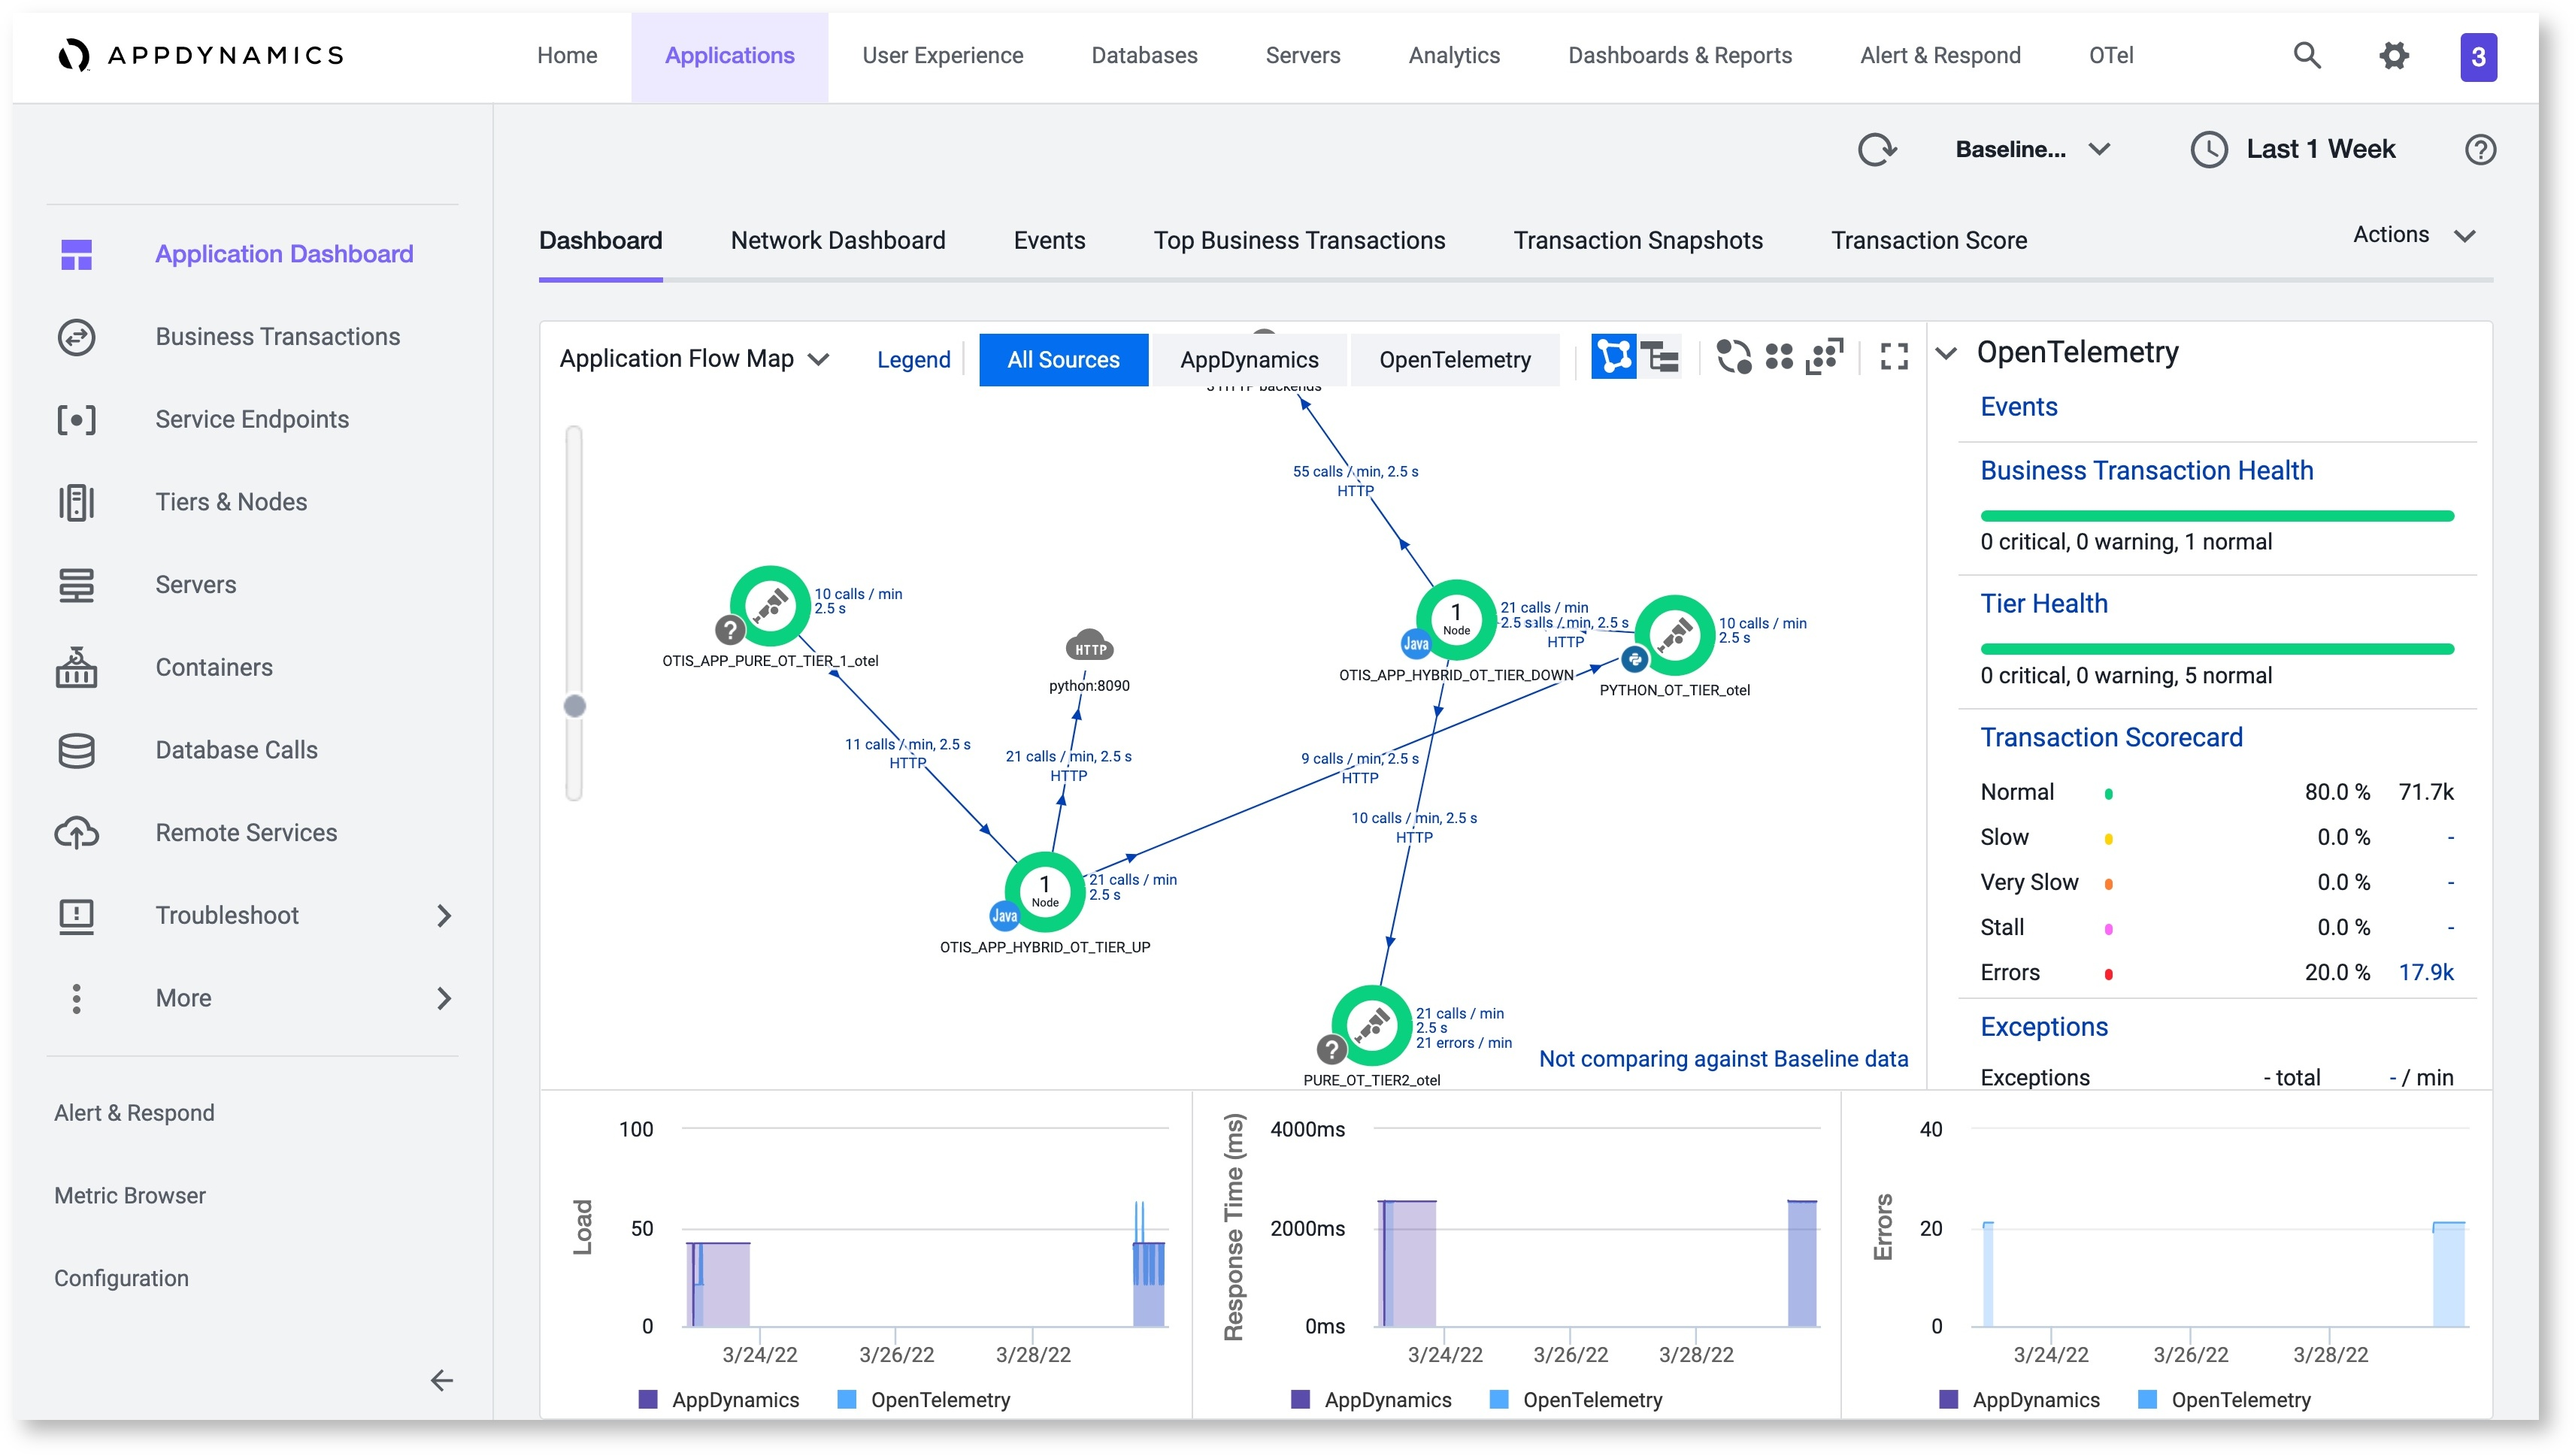
\includegraphics[width=15cm]{obrazky-figures/Application_Dashboard.jpeg}
  \caption{Ukázka webového rozhraní AppDynamics\protect\footnotemark}
  \label{fig:dynamics}
\end{figure}
\footnotetext{Obrázek byl převzat z~webu \url{https://cdn.brandfolder.io/50KQXSAT/at/hfm5nm7rqbrn6298rbrtqbf/Application_Dashboard.jpeg} [25.12.2022]}

\subsection{Poskytovatel cloudových služeb Amazon Web Services (AWS)}
Firma AWS si vytvořila vlastní distribuci OpenTelemetry s~podporou původních tvůrců. Rozšířila systém o~sběr metadat z~cloudových zdrojů AWS a jejich služeb. Můžeme tedy korelovat data o~výkonu aplikace a o~infrastruktuře, na které běží, tím pádem zkrátíme průměrnou dobu do vyřešení problému, pokud nastane. Pomocí AWS distribuce můžeme sbírat telemetrická data, když aplikace běží v~následujících prostředí.
    \begin{itemize}
        \item{Amazon Elastic Compute Cloud (EC2)}
        \item{Amazon Elastic Container Service (ECS) a Amazon Elastic Kubernetes Service (EKS)}
        \item{AWS Fargate}
        \item{AWS Lambda}
    \end{itemize}

Je zde ale jedna nevýhoda, musíme využít monitorovacích nástrojů od AWS (AWS X-Ray, Amazon CloudWatch, Amazon Managed Service for Prometheus) nebo jejich partnerů.

\subsection{Elastic}
Elastic je monitorovací nástroj, který je úplně zdarma. Umožní nám rychle vizualizovat všechna telemetrická data ve webovém rozhraní, data ze systému OpenTelemetry pomocí Elastic Stacku. 

Jelikož podporuje nativně OpenTelemetry protokol, stačí nám pouze v~exportéru nastavit koncový bod monitorovacího nástroje a autorizaci pomocí vygenerovaného Api klíče.

\begin{figure}[H]
  \centering
  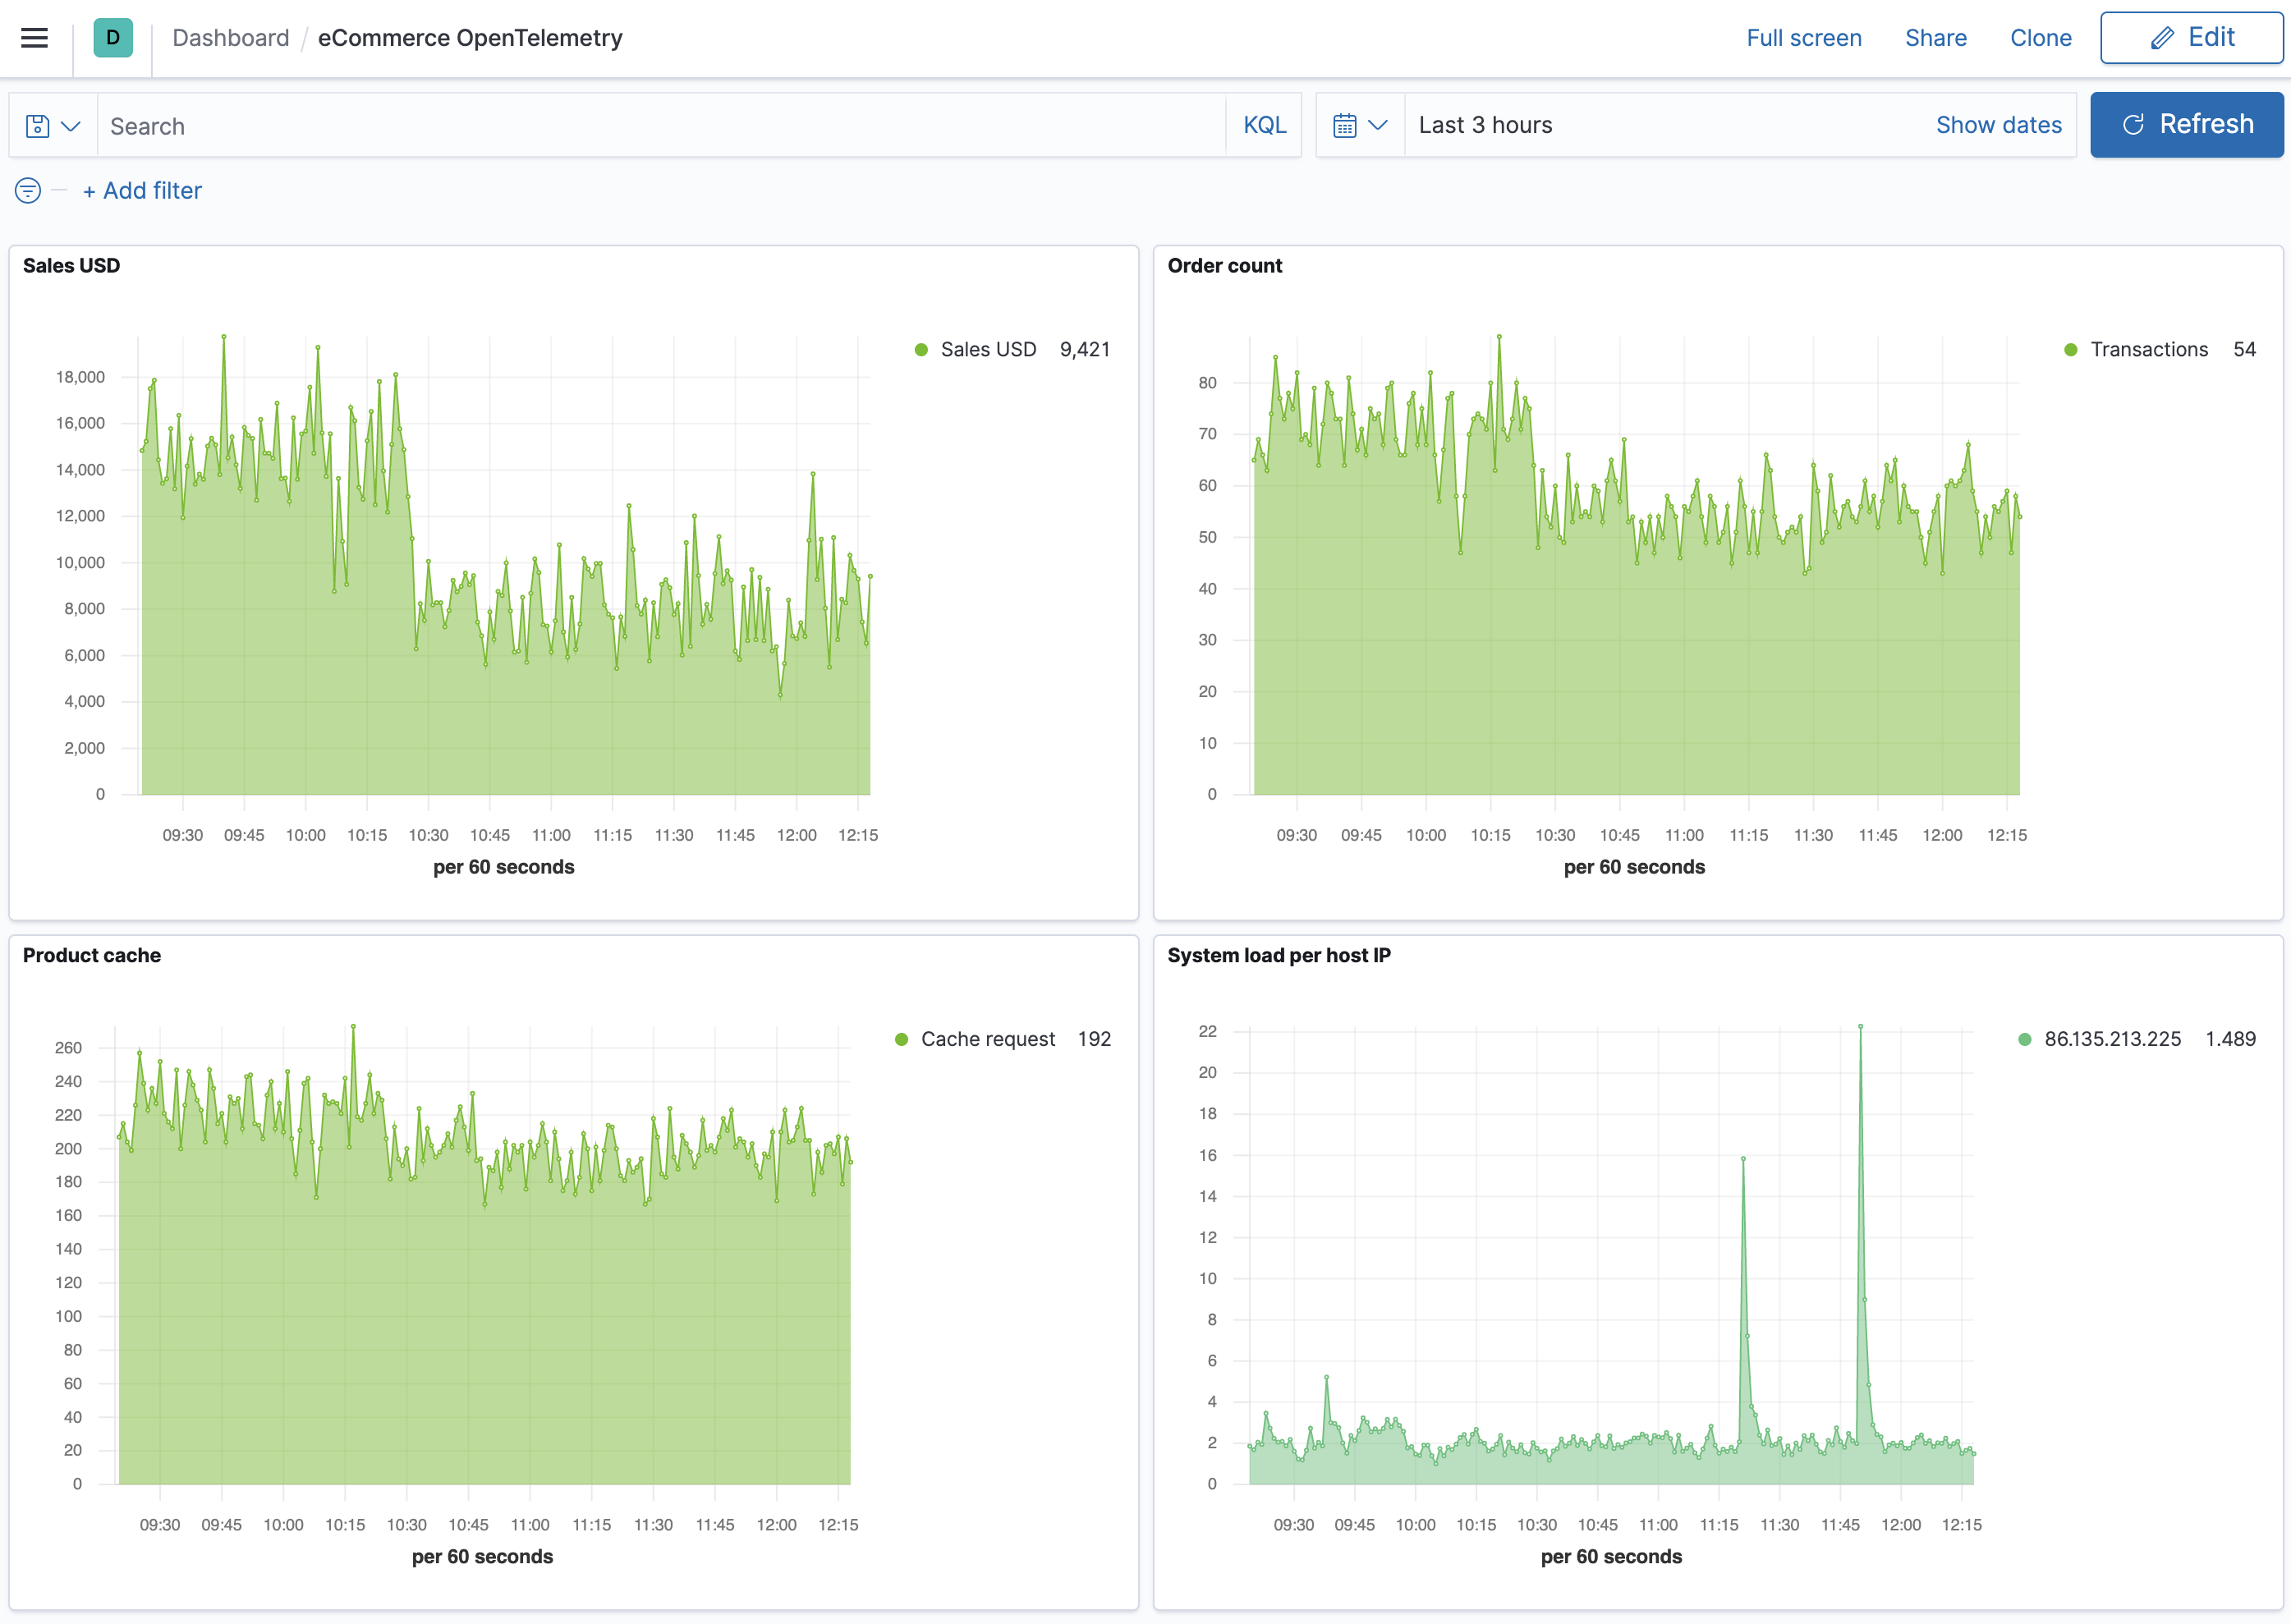
\includegraphics[width=13.5cm]{obrazky-figures/elastic.png}
  \caption{Ukázka webového rozhraní Elastic zobrazující metriky\protect\footnotemark}
  \label{fig:elastic}
\end{figure}
\footnotetext{Obrázek byl převzat z~webu \url{https://www.elastic.co/guide/en/apm/guide/current/legacy/guide/images/ecommerce-dashboard.png} [26.12.2022]}

\subsection{Projekt Grafana Labs}
Monitorovací nástroj s~otevřeným zdrojovým kódem. Podporuje vizualizaci všech telemetrických dat, které nabízí systém OpenTelemetry. Zobrazit si vizualizace můžeme ve webovém rozhraní. Nabízí zdarma doživotní přístup pro jednoho uživatele při maximální zátěži 10 tisíc aktuálně zpracovávaných požadavků a 50GB dat pro záznamy.

Telemetrická data můžeme odesílat pomocí protokolu OpenTelemetry a to třemi způsoby.
\begin{itemize}
    \item{Pomocí kolektoru, kde v~rozšíření nastavíme autentizaci a v~exportéru na ní odkážeme.}
    \item{Odesílat data přímo z~aplikace do Grafana Cloud. Doporučuje se pouze pro testování.}
    \item{Pomocí Grafana agenta, který poskytuje koncový bod OTLP pro příjem dat. Zatím je tato funkce v~raném vývoji, a proto se nedoporučuje použít v~produkci.}
\end{itemize}

\subsection{Firma Splunk}
Softwarová firma Splunk vyvíjí monitorovací nástroje podporující telemetrická data ze systému OpenTelemetry. Splunk APM je monitorovací nástroj pro vizualizaci dat z~aplikací a Splunk Infrastructure Monitoring je monitorovací nástroj pro vizualizaci dat o~infrastruktuře na které mohou aplikace běžet.

Splunk také vyvinul vlastní knihovny pro automatický sběr telemetrických dat z~aplikace pro programovací jazyky Java a Python.

Pro odesílání dat na monitorovací nástroj máme předpřipravený kolektor od firmy Splunk, jež podporuje protokoly pro příjem dat, jako jsou OpenTelemetry protokol, Jaeger, Zipkin a Prometheus.


\chapter{Testovací prostředí}

Systém OpenTelemetry podporuje velké množství programovacích jazyků a proto jsem se rozhodl použít demo aplikaci přímo od tvůrců systému OpenTelemetry. Aplikace je navržena pomocí mikroslužeb\footnote{Jedná se o~architekturu, kde výsledná aplikace je rozdělena do několika menších. Přináší to výhodu, že na každé části může pracovat jiný tým, který si může zvolit vlastní nástroje k~vývoji.}. Díky této architektuře využijeme většinu programovacích jazyků, podporovaných systémem OpenTelemetry.

\section{Demo aplikace}
Aplikace představuje on-line obchod s~hvězdářskými potřebami, kde uživatel může přidat produkt do košíku, vybrat měnu, ve které bude nakupovat, a košík s~produkty objednat.


\begin{figure}[H]%
    \centering
    \subfloat{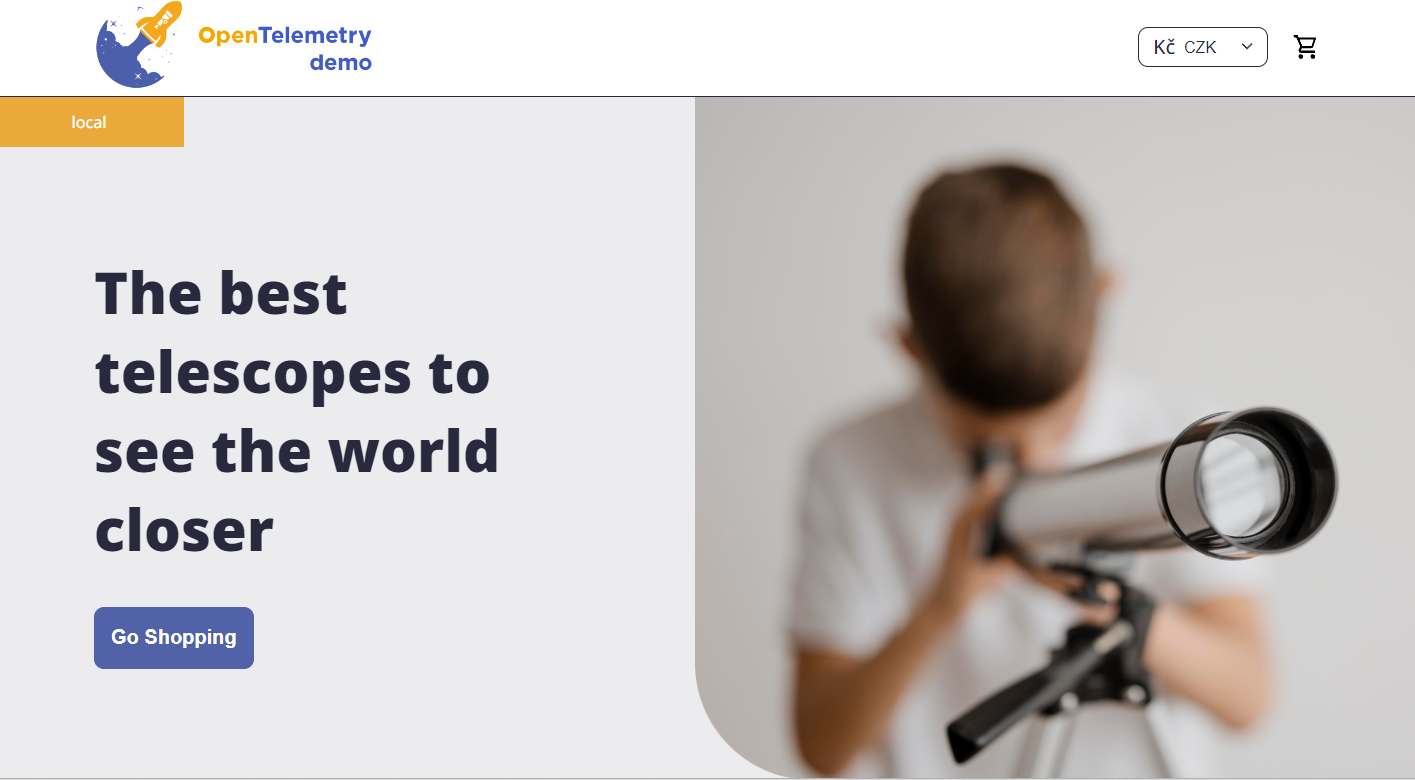
\includegraphics[width=7.2cm]{obrazky-figures/shop1.png}}%
    \qquad
    \subfloat{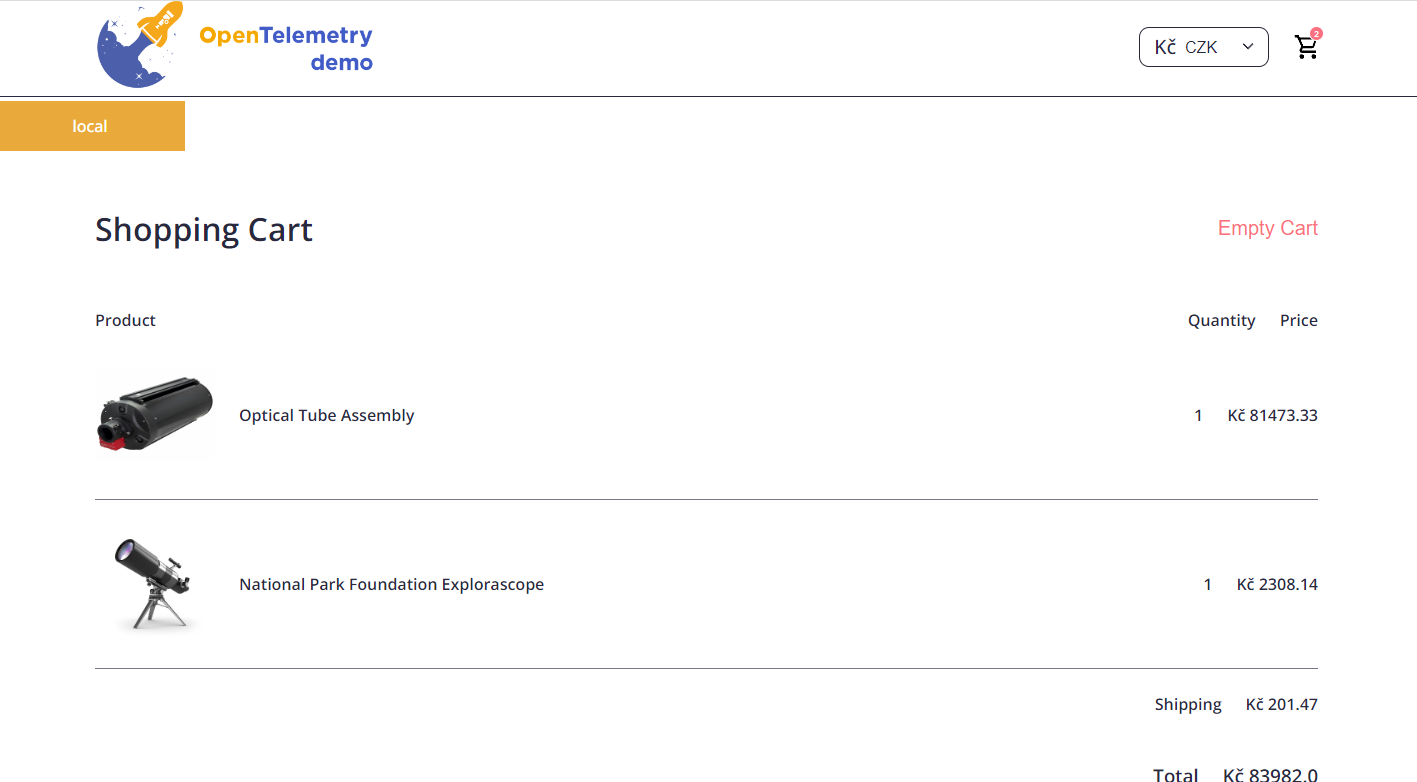
\includegraphics[width=7.2cm]{obrazky-figures/shop2.png}}%
    \caption{Ukázka obchodu}%
    \label{fig:example}%
\end{figure}

\subsection{Architektura aplikace}
Aplikace je založena na architektuře mikroslužeb. Skládá se z~14 služeb, kde každá obstarává určitou funkcionalitu webové aplikace a je napsána jinou technologií, aby se pokryla větší část knihoven pro generování telemetrických dat systému OpenTelemetry.

Nachází se zde ještě jedna služba, která má simulovat uživatele a jejich pohyb po webové aplikaci.

\begin{figure}[H]
  \centering
  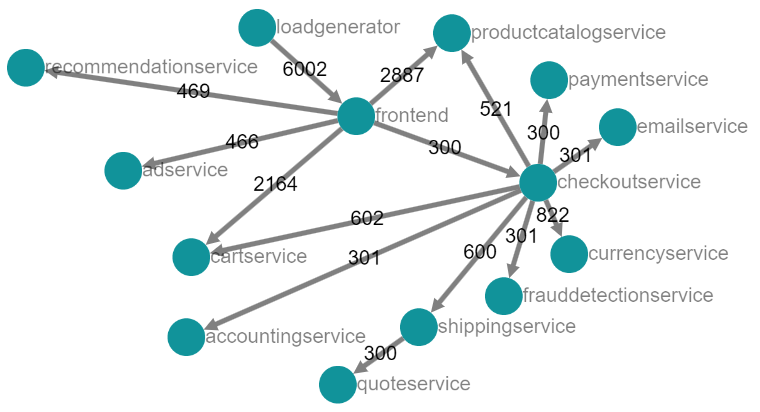
\includegraphics[width=15cm]{obrazky-figures/demoArchitecture.png}
  \caption{Ukázka architektury aplikace a komunikace mezi jednotlivými službami}
  \label{fig:demoArchitecture}
\end{figure}

Na obrázku \ref{fig:demoArchitecture} vidíme jednotlivé služby, komunikaci mezi nimi a počet požadavků. Směr šipek nám udává, která služba odeslala požadavek. Můžeme si všimnout, že danou architekturu nám vykreslil monitorovací nástroj Jaeger. Dále si popíšeme hlavní služby podrobněji.
\begin{itemize}
        \item{\textbf{Ad Service}}
        \item[]
        Jedná se o~službu napsanou v~jazyce Java s~použitím automatického generování telemetrických dat. Tato služba určuje vhodné reklamy, jež se mají uživateli zobrazovat. Používáme knihovnu i pro manuální generování telemetrických dat pro doplnění například atributů do operací.
        \item{\textbf{Cart Service}}
        \item[]
        Jedná se o~službu napsanou v~jazyce .NET s~použitím automatického generování telemetrických dat. Tato služba uchovává položky vložené do košíku.
        \item{\textbf{Checkout Service}}
        \item[]
        Jedná se o~službu napsanou v~jazyce Go s~použitím automatického generování telemetrických dat. Tato služba je zodpovědná za zpracování objednávek od uživatele.
        \item{\textbf{Currency Service}}
        \item[]
        Jedná se o~službu napsanou v~jazyce C++. Tato služba se stará o~převod jedné měny na jinou.
        \item{\textbf{Email Service}}
        \item[]
        Jedná se o~službu napsanou v~jazyce Ruby s~použitím automatického generování telemetrických dat. Tato služba odesílá email s~potvrzením objednávky.
        \item{\textbf{Fraud Detection Service}}
        \item[]
        Jedná se o~službu napsanou v~jazyce Kotlin s~použitím automatického generování telemetrických dat. Tato služba má na starost detekci podvodných objednávek.
        \item{\textbf{Frontend}}
        \item[]
        Jedná se o~službu napsanou v~jazyce JavaScript s~použitím automatického generování telemetrických dat. Tato služba je zodpovědná za poskytnutí uživatelského rozhraní a komunikaci s~API.
        \item{\textbf{Payment Service}}
        \item[]
        Jedná se o~službu napsanou v~jazyce JavaScript s~použitím automatického generování telemetrických dat. Tato služba je zodpovědná za zpracování plateb platební kartou a kontrolu validity platební karty.
        \item{\textbf{Product Catalog Service}}
        \item[]
        Jedná se o~službu napsanou v~jazyce Go s~použitím automatického generování telemetrických dat. Tato služba zodpovídá za práci s~produkty v~obchodě. 
        \item{\textbf{Quote Service}}
        \item[]
        Jedná se o~službu napsanou v~jazyce PHP. Tato služba počítá poštovné na základě položek obsažené v~košíku.
        \item{\textbf{Recommendation Service}}
        \item[]
        Jedná se o~službu napsanou v~jazyce Python s~použitím automatického generování telemetrických dat. Tato služba doporučuje produkty pro uživatele na základě jeho aktivity.
        \item{\textbf{Shipping Service}}
        \item[]
        Jedná se o~službu napsanou v~jazyce Rust. Tato služba poskytuje informace o~ceně a informace o~přepravě objednávky.
    \end{itemize}

\subsection{Simulace uživatelů}
Simulaci chování uživatele na webové aplikaci zajišťuje služba \textit{Load Generator}. Tato služba je napsaná v~jazyce Python a pro generování požadavků využívá knihovnu \textit{Locust}\footnote{Knihovna Locust \url{https://docs.locust.io/en/stable/writing-a-locustfile.html} [30.12.2022]}

\begin{figure}[H]
  \centering
  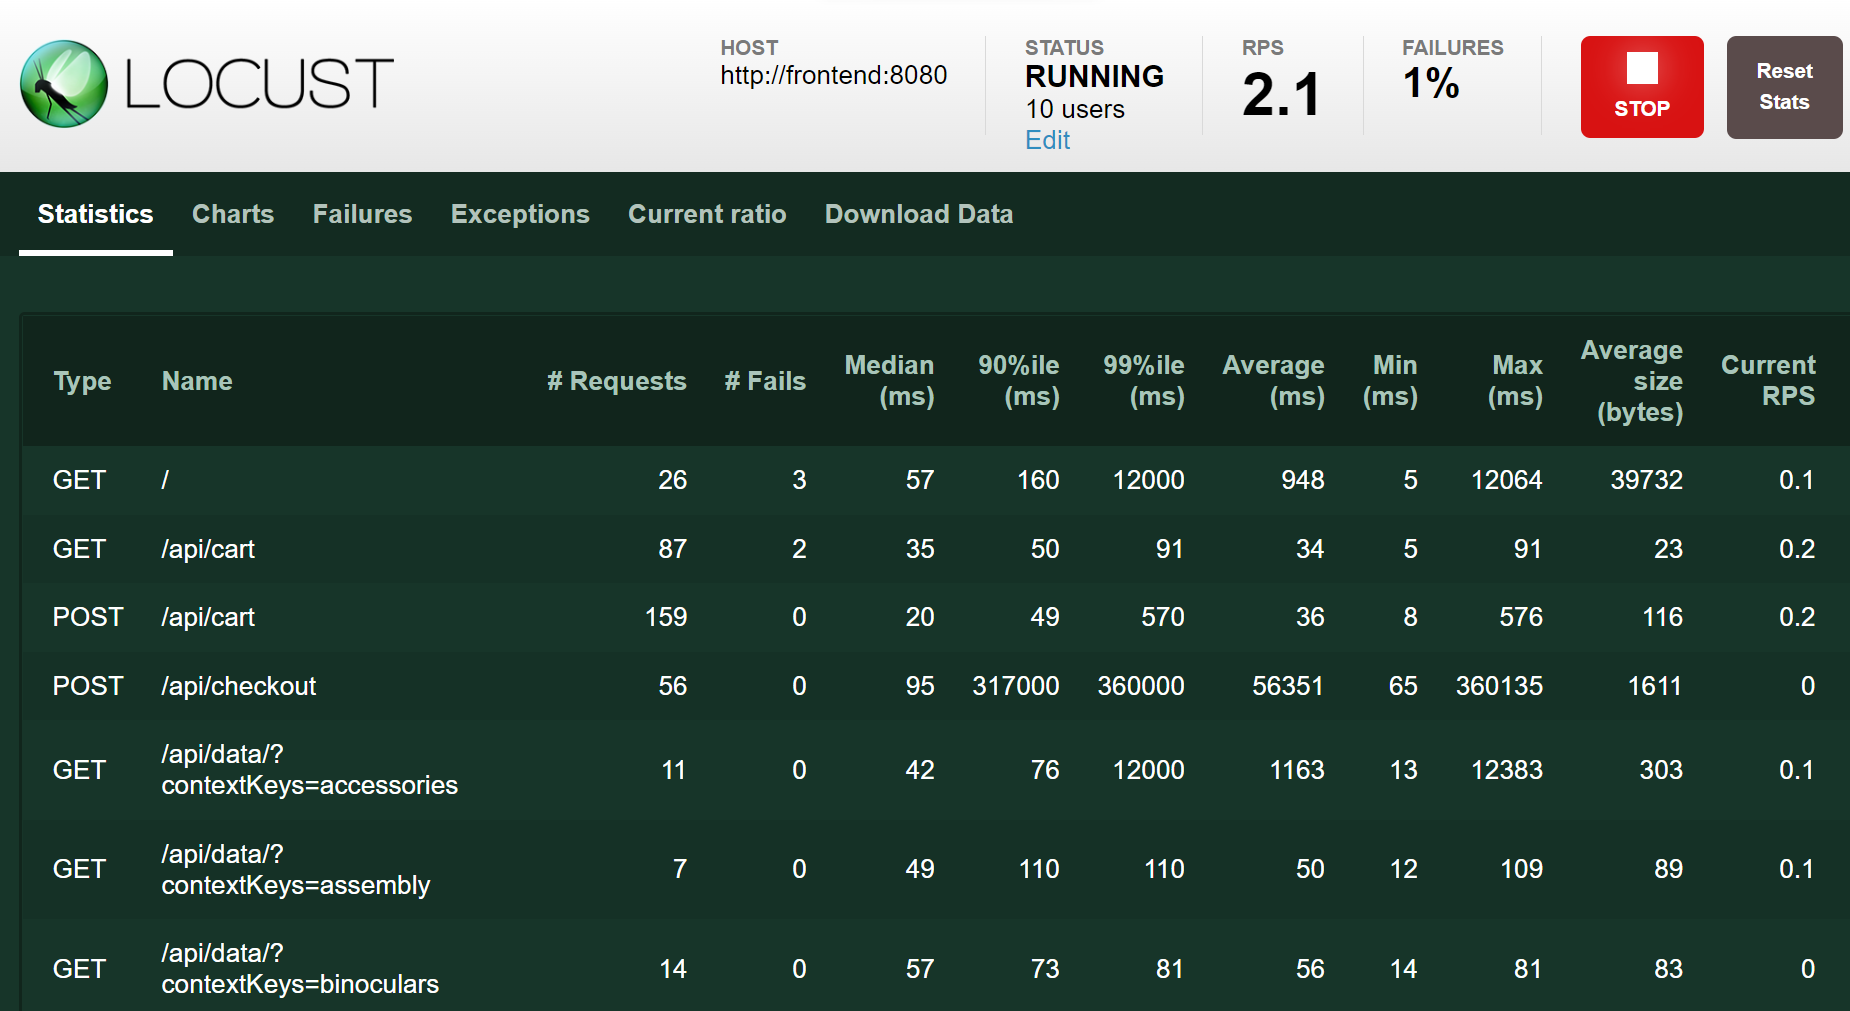
\includegraphics[width=15cm]{obrazky-figures/locust.png}
  \caption{Ukázka webového rozhraní pro simulaci uživatelů}
  \label{fig:locust}
\end{figure}

Na obrázku \ref{fig:locust} vidíme požadavky, které generujeme a jejich statistiky. V~horní liště můžeme měnit počet simulovaných uživatelů. Nyní vidíme, že na webu simulujeme chování 10 uživatelů. Vedle se nachází hodnota, jež udává počet požadavků za sekundu a procento chybných požadavků. Můžeme zde generování požadavků přerušit nebo vymazat statistiky.

\section{Testovací prostředí}
Pro testování jsem oddělil aplikaci a kolektor s~monitorovacími nástroji na dva různé servery. Umožní nám to odchytávat komunikaci a zkoumat jednotlivé pakety, zahlcení sítě komunikací při odesílání dat kolektoru a mnoho dalších způsobů testování daného systému.

Architekturu testovacího prostředí můžeme lehce změnit díky využití kontejnerizace. Každá služba má vlastní kontejner a tak není problém nasadit danou část na odlišný server.

\begin{figure}[H]
  \centering
  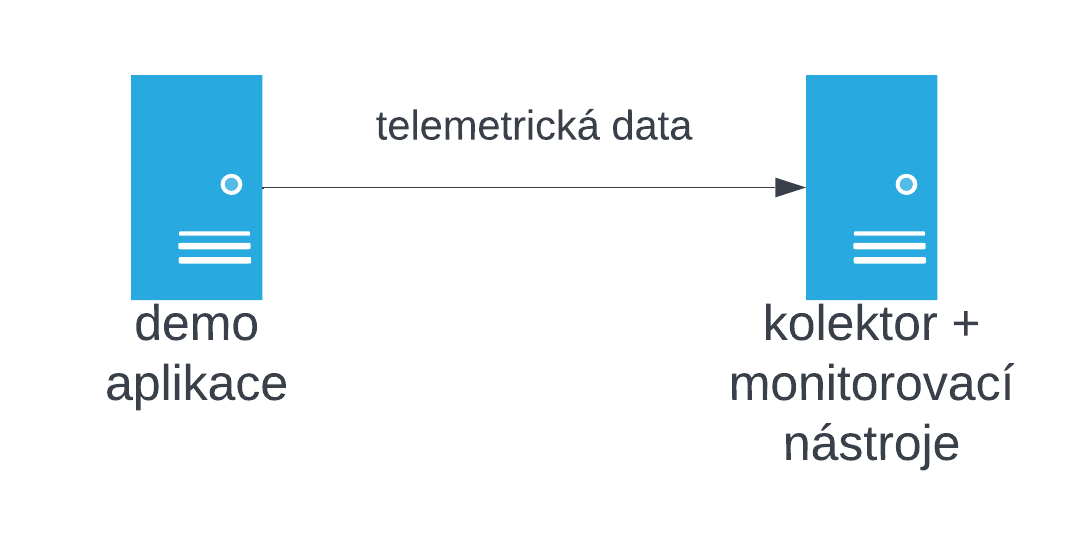
\includegraphics[width=11cm]{obrazky-figures/architectureServers.png}
  \caption{Ukázka testovacího prostředí}
  \label{fig:serverArchitecture}
\end{figure}

Zachytával jsem pakety v~různých časových intervalech a při různém počtu požadavků, které jsem ovlivňoval pomocí změny počtu simulovaných uživatelů.

\begin{table}[H]
  \centering
   \begin{tabular}{|l|c|c|c|}
     \hline
      & \multicolumn{3}{c|}{\bfseries Doba v~minutách} \\
     \cline{2-4}
     \bfseries Počet uživatelů & \bfseries 10 & \bfseries 30 & \bfseries 60\\
     \hline
     1 & 11 250 & 28 765 & 57 528\\
     10 & 21 310 & 64 246 & 128 031\\
     50 & 44 599 & 136 560 & 245 422\\
     \hline
    \end{tabular}
    \caption{Počet zachycených paketů}
    \label{tab:pakety}
\end{table}

V~tabulce \ref{tab:pakety} vidíme celkový počet zachycených paketů. Pro sběr komunikace jsem měl nastavený filtr na porty 4317 a 4318. V~počtech paketů jsou započítána odesílaná telemetrická data a potvrzení od serveru o~jejich přijetí.



\section{Monitorovací nástroje}
Telemetrická data vizualizujeme pomocí tří monitorovacích nástrojů. Stopy odesíláme do monitorovacího nástroje \textit{Jaeger} a metriky do nástroje \textit{Prometheus}. Poté všechna telemetrická data využívá nástroj \textit{Grafana}.

\subsection{Prometheus}
Monitorovací nástroj Prometheus nám zobrazuje metriky. Vidíme všechny přijaté metriky a můžeme si je vizualizovat do panelů podle našich preferencí. Můžeme si je zobrazit jako hodnoty nebo v~grafu,  jak se vyvíjely v~čase. 

\begin{figure}[H]
  \centering
  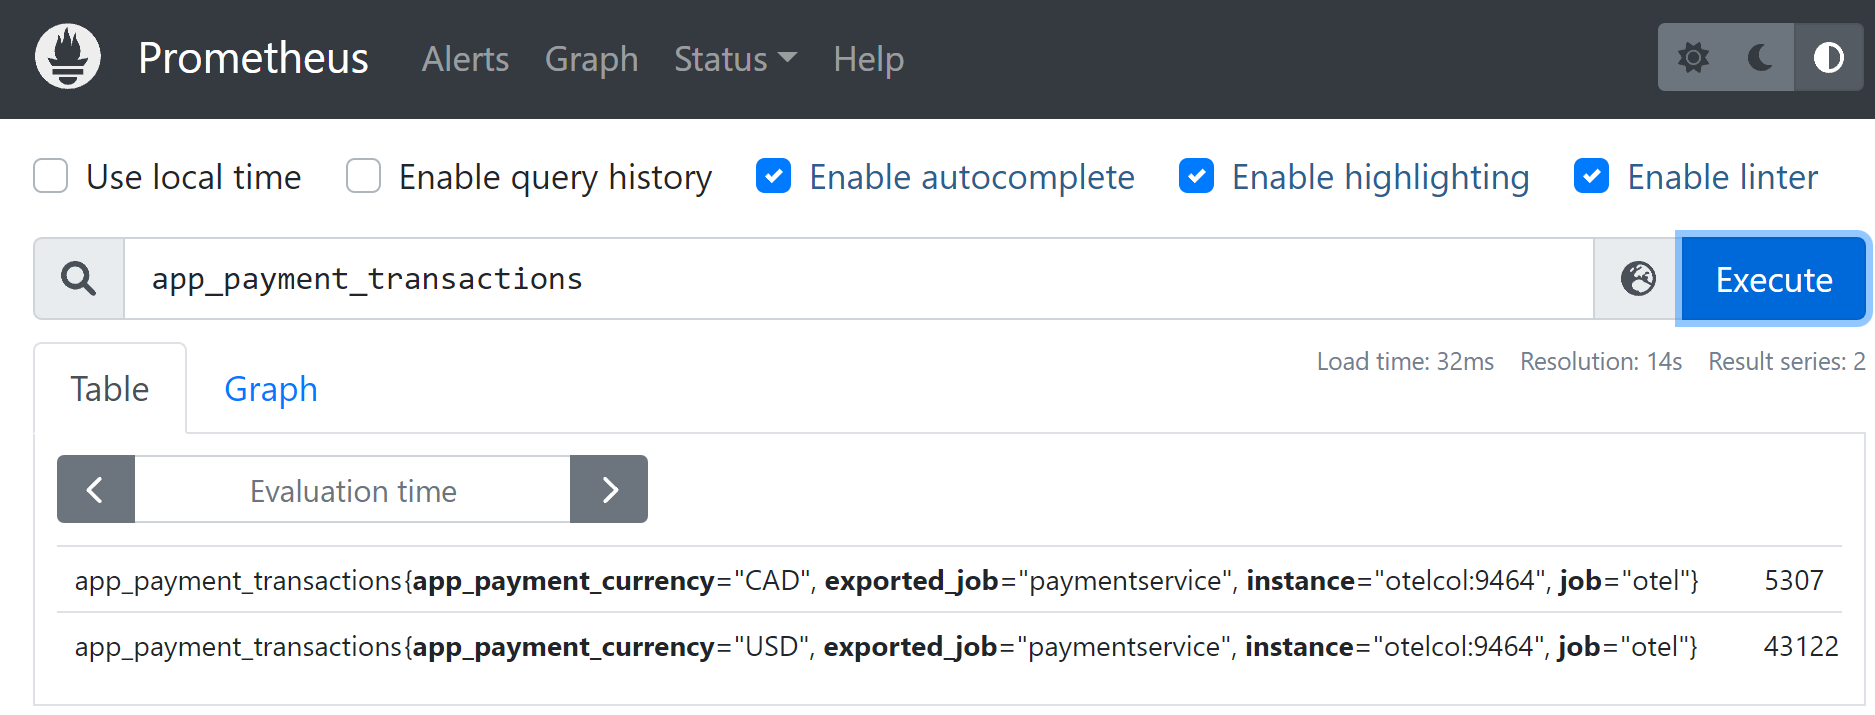
\includegraphics[width=15cm]{obrazky-figures/prometheusTable.png}
  \caption{Ukázka monitorovacího nástroje Prometheus}
  \label{fig:prometheusTable}
\end{figure}

Na obrázku \ref{fig:prometheusTable} vidíme metriku, kde je vypsaná celková částka, která byla utracena za objednávky ve stejné měně.

\subsection{Jaeger}
Monitorovací nástroj Jeager nám umožňuje vizualizovat distribuované stopy. Nabízí výpis stop pro jednotlivé služby, porovnání dvou stop, ukázku architektury aplikace nebo monitorování služeb. 

\begin{figure}[H]
  \centering
  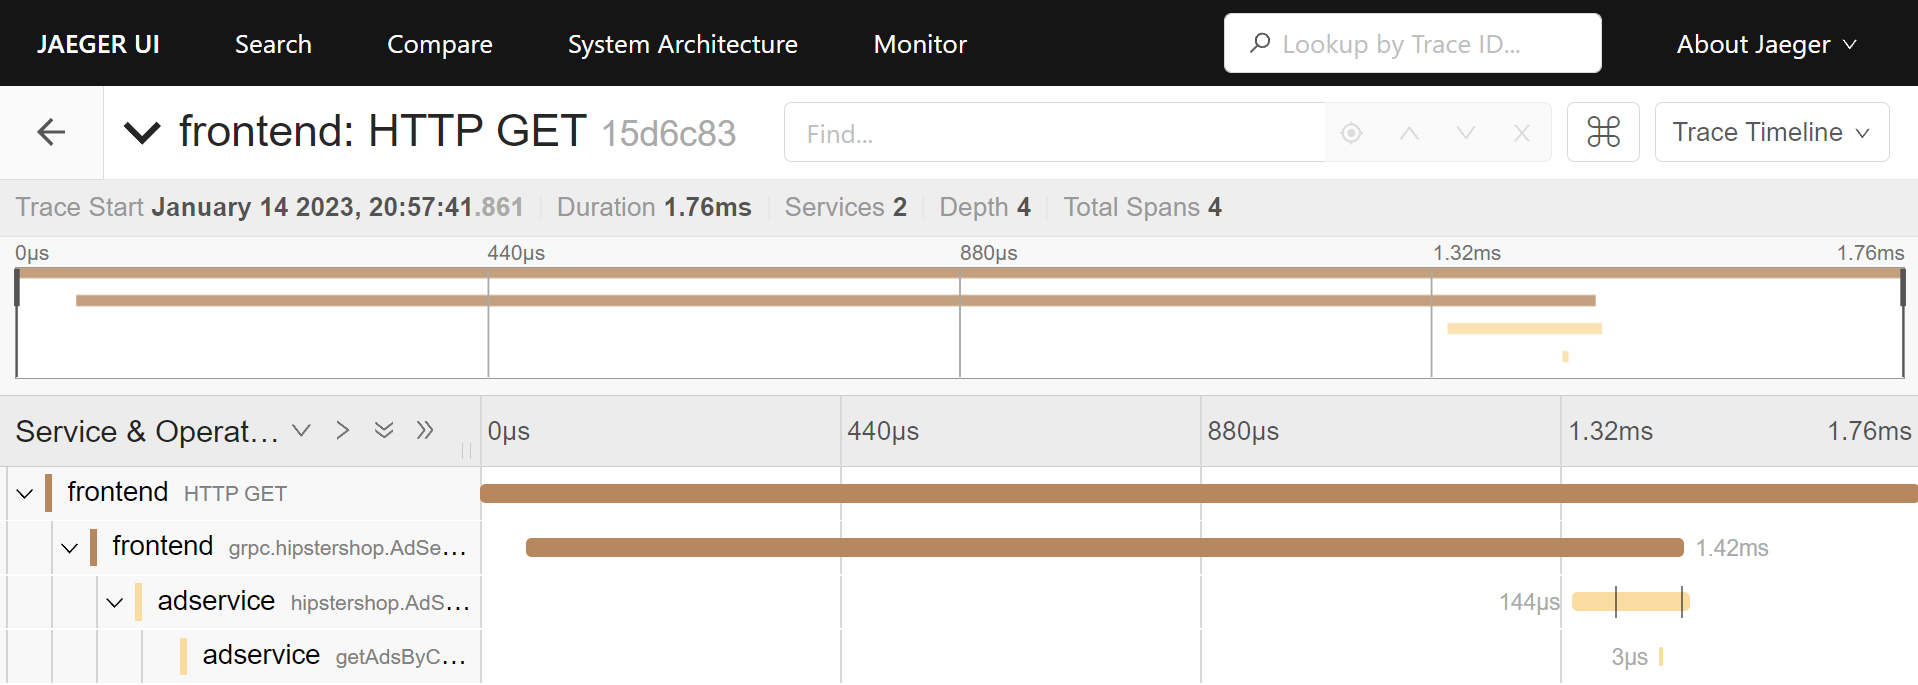
\includegraphics[width=15cm]{obrazky-figures/jaegerTrace.png}
  \caption{Ukázka monitorovacího nástroje Jaeger}
  \label{fig:jaegerTrace}
\end{figure}

Na obrázku \ref{fig:jaegerTrace} vidíme distribuovanou stopu se čtyřmi operacemi a informacemi, které nám mohou být užitečné při hledání problému nebo optimalizaci programu, jako je například doba trvání jednotlivých operací.

\subsection{Grafana}

Monitorovací nástroj Grafana nám umožňuje vizualizovat všechna telemetrická data, jež podporuje systém OpenTelemetry. Uživateli, který bude sledovat telemetrická data, umožňuje vytvořit nástěnky s~panely podle jeho preferencí.

\begin{figure}[H]
  \centering
  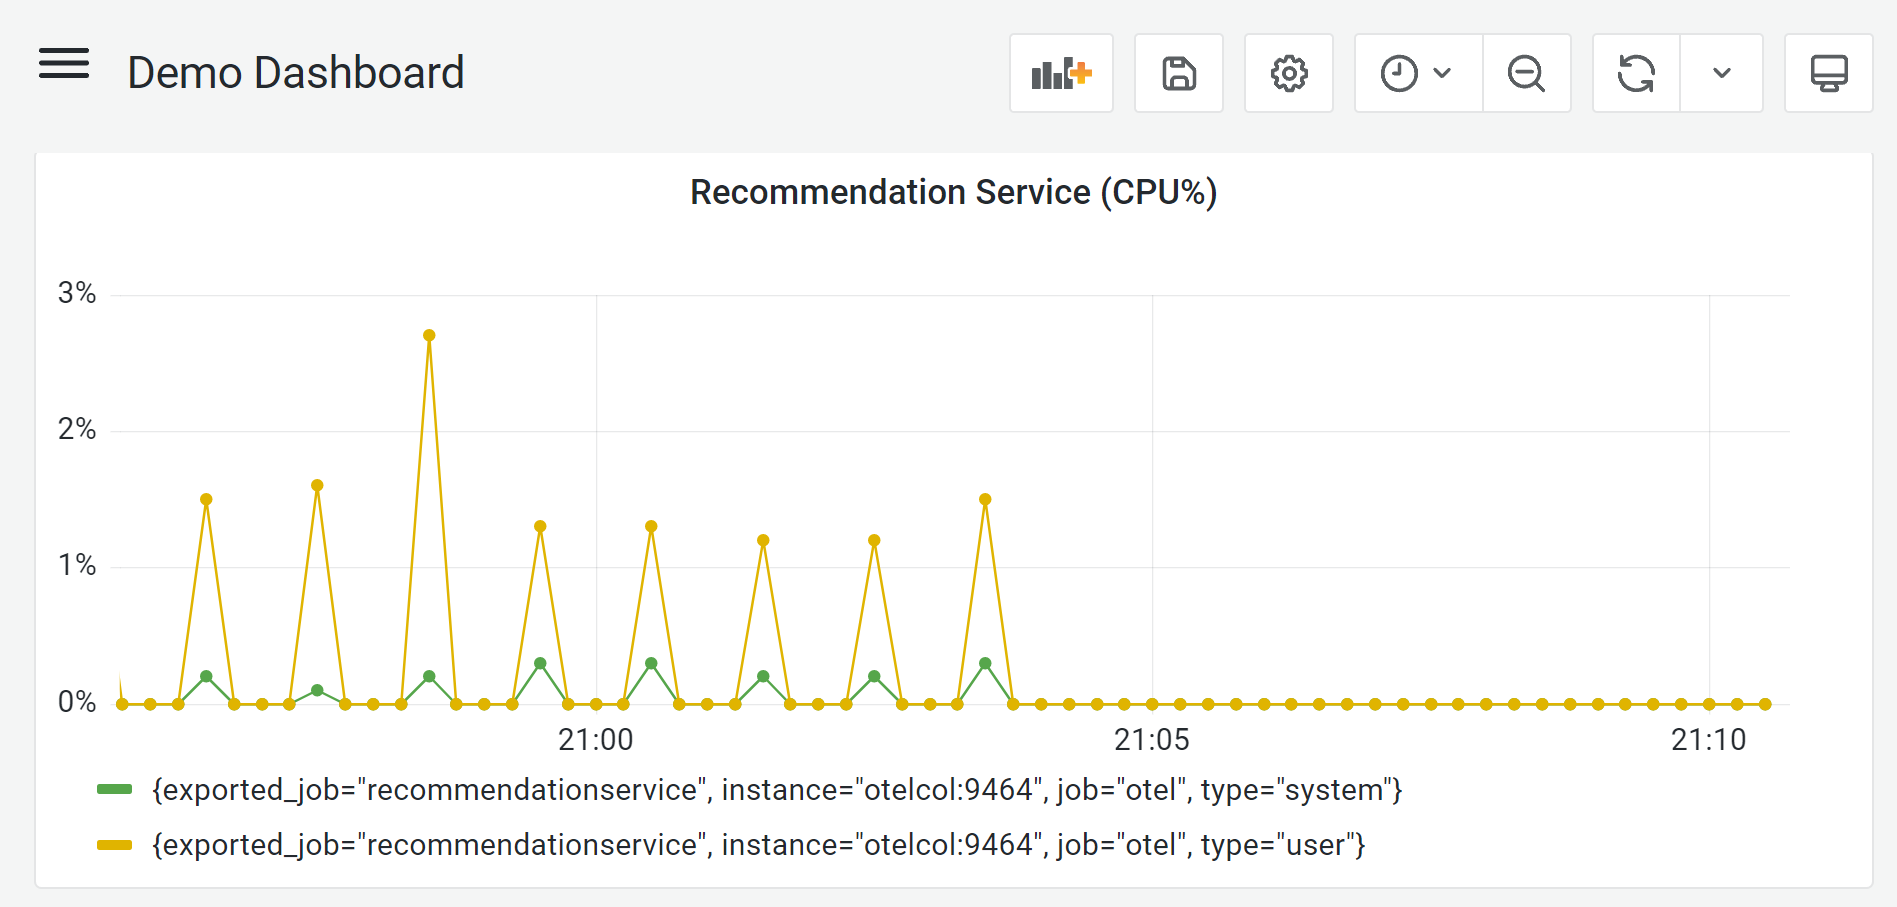
\includegraphics[width=15cm]{obrazky-figures/grafana.png}
  \caption{Ukázka monitorovacího nástroje Grafana}
  \label{fig:grafana}
\end{figure}

Na obrázku \ref{fig:grafana} vidíme graf, který znázorňuje využití procesoru službou \textit{Recommendation Service}.

\chapter{Experimenty s~testovacím prostředím}
V~této kapitole si ukážeme jak zachytit a přečíst pakety systému OpenTelemetry. Provedeme experimenty v~testovacím prostředí a podíváme se, jak telemetrická data vypadají. Cílem této kapitoly je získat představu, jaké události můžeme detekovat pomocí dat ze systému OpenTelemetry a jak data vypadají na síti.

\section{Zachycení komunikace}
Pro zachycení komunikace využíváme nástroj \texttt{tcpdump}\footnote{Oficiální stránky nástroje tcpdump \url{https://www.tcpdump.org/} [28.03.2023]}, který slouží pro sběr a analýzu síťové komunikace v~reálném čase a je dostupný na většině Unixových operačních systémech.

\begin{listing}[H]
    \begin{minted}{bash}
tcpdump -i enp2s0 'port 4317 or 4318' -w packetsOTLP.pcap
\end{minted}
    \caption{Příkaz pro zachycení komunikace}
    \label{lst:tcpdump}
\end{listing}

Ve výpisu \ref{lst:tcpdump} vidíme zachycení komunikace na rozhraní \texttt{enp2s0}. Filtrujeme komunikaci pomocí portů 4317 a 4318, na kterých se nachází komunikace systému OpenTelemetry, a ukládáme zachycenou komunikaci do souboru \texttt{packetsOTLP.pcap}.


\section{Čtení dat z~komunikace}

Zachycenou komunikaci přečteme za využití nástroje \texttt{Wireshark}\footnote{Oficiální stránky nástroje Wireshark \url{https://www.wireshark.org/} [28.03.2023]}. Používá se ke sběru a analýze paketů, ale na rozdíl od nástroje \texttt{tcpdump} nabízí uživateli přívětivé grafické rozhraní.

Systém OpenTelemetry vyžívá protokoly gRPC a HTTP2. Pro serializaci dat využívá Protocol Buffers ve výchozím nastavení. Wireshark v~základním nastavení nedokáže zobrazit zachycená data v~čitelné podobě pro člověka. Musíme přidat \texttt{.proto} soubory, pomocí kterého Wireshark deserializuje data do čitelné podoby pro člověka.

\begin{listing}[H]
    \begin{minted}{proto}
syntax = "proto3";

package opentelemetry.proto.common.v1;

message KeyValue {
  string key = 1;
  AnyValue value = 2;
}
\end{minted}
    \caption{Definice souboru .proto ze systému OpenTelemetry pro strukturu klíč-hodnota}
    \label{lst:proto}
\end{listing}

Systém OpenTelemetry poskytuje veřejně soubory .proto pro veškerou jejich komunikaci. Najdeme je na úložišti GitHub\footnote{Repositář s~.proto soubory \url{https://github.com/open-telemetry/opentelemetry-proto} [12.04.2023]}. Vložíme je do Wiresharku v~záložce \textbf{Edit > Preferences > Protocols > ProtoBuf}, kde vložíme cestu k~souborům a zaklikneme políčko \textbf{Load all files}. Poté nastavíme komunikaci na HTTP2 na určitém portu a to pomocí \textbf{Analyze > Decode As..}, kde přidáme novou položku s~hodnotami TCP protokol a port, který je v~našem případě 4317 a HTTP2 protokol.

\begin{figure}[H]
  \centering
  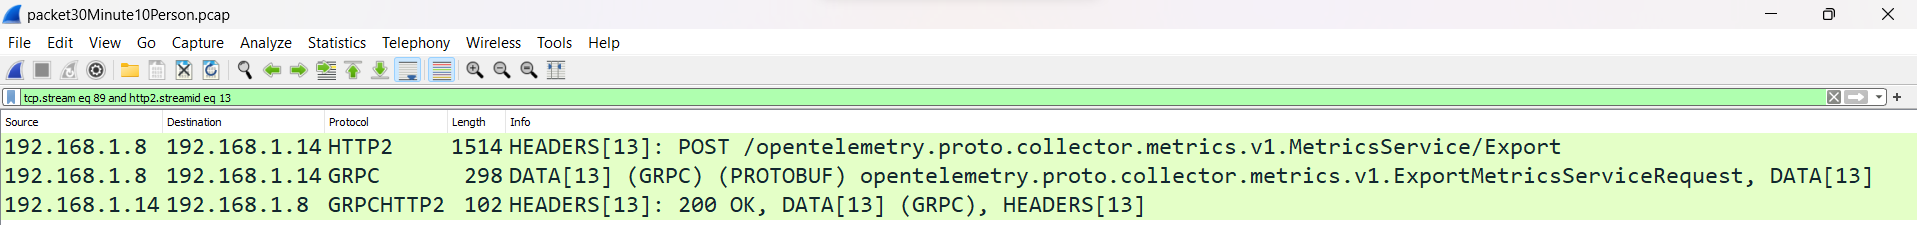
\includegraphics[width=15cm]{obrazky-figures/wireshark.png}
  \caption{Ukázka jednoho toku komunikace}
  \label{fig:wireshark}
\end{figure}

\begin{listing}[H]
    \begin{minted}{json}
{
  "name": "process.runtime.dotnet.assemblies.count",
  "description": "The number of .NET assemblies that are currently loaded.",
  "gauge": {
    "data_points": [
      {
        "start_time_unix_nano": "1673739808162277500",
        "time_unix_nano": "1673790268036106100",
        "as_int": "8"
      }
    ]
  }
}
\end{minted}
    \caption{Ukázka metriky ze zachycené komunikace ve Wiresharku za využití mapování na JSON}
    \label{lst:protoMetrika}
\end{listing}


\section{Experimenty}
Účelem experimentů je nasimulovat nežádoucí stavy v~testovacím prostředí, se kterými se můžeme setkat při provozu aplikace. Experimenty budeme provádět na testovacím prostředí, které je popsané v~tabulce \ref{tab:konf}.

\begin{table}[H]
\begin{tabular}{|l|l|l|}
\hline
               & \textbf{Testovací aplikace}  & \textbf{Kolektor + Monitorovací nástroje} \\ \hline
\textbf{Model} & Acer Aspire VN7-572G & Raspberry Pi 4 Model B Rev 1.4 \\ \hline
\textbf{CPU}   & Intel(R) Core(TM) i5-6200U @ 2.30GHz & Broadcom BCM2711 \\ \hline
\textbf{RAM}   & 8 GiB DDR4 & 8 GiB LPDDR4  \\ \hline
\end{tabular}
\caption{Konfigurace testovacího prostředí}
\label{tab:konf}
\end{table}

\subsection{Experiment č. 1: Výpadek mikroslužby}

Testovací aplikace je navržena pomocí architektury mikroslužeb, kde každá mikroslužba může běžet na vlastním stroji. K~plné funkcionalitě aplikace musí všechny mikroslužby běžet. Tímto experimentem testujeme nedostupnost mikroslužby z~důvodu výpadku stroje, na kterém běží, přerušení síťového spojení a mnoho dalších výpadků mikroslužby.

\subsubsection{Navození nežádoucího stavu}

Nežádoucí stav navodíme vypnutím jedné mikroslužby. Díky využití technologie Docker kontejnerů, kde každá mikroslužba běží ve vlastním kontejneru, vypneme pouze kontejner s~danou mikroslužbou. Pro náš experiment vypneme službu \texttt{feature-flag-service}.

\subsubsection{Výsledek}

V~monitorovacím nástroji Jeager po vybrání mikroslužby, která se snaží o~komunikaci s~nedostupnou mikroslužbou, hned vidíme v~úvodním grafu, že některé stopy obsahují chybovou hlášku.

\begin{figure}[H]
  \centering
  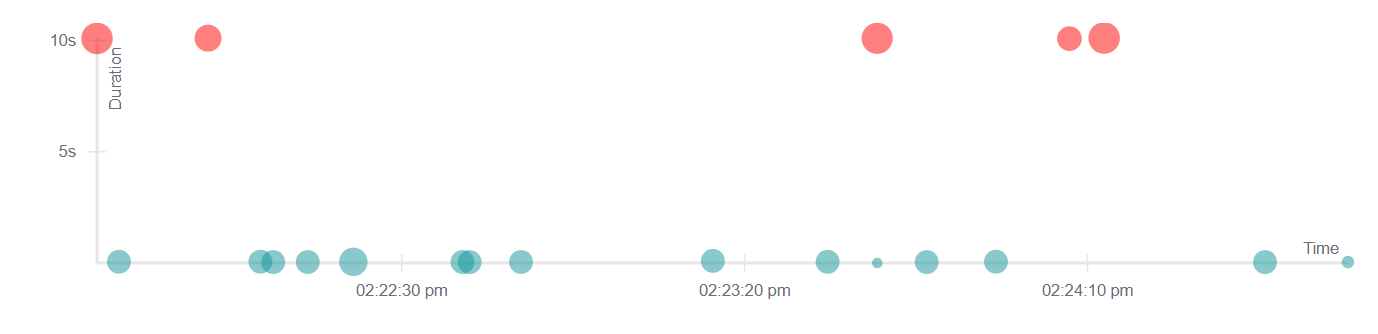
\includegraphics[width=15cm]{obrazky-figures/jeagerGraf.png}
  \caption{Úvodní graf ukazující čas přijatý stopy a její délku trvání}
  \label{fig:jeagerGraf}
\end{figure}

Na obrázku \ref{fig:jeagerGraf} vidíme graf s~posledními 20 přijatými stopami. Můžeme si všimnout pěti stop, které jsou označeny červenou barvou, která značí stopu s~chybou. Nejen podle červené barvy vidíme, že je něco v~nepořádku. Délka trvání stopy nám může také pomoci při hledání chyby. Vidíme, že stopy s~chybou trvají okolo 10 sekund a zbylé trvají necelou sekundu.

\begin{figure}[H]
  \centering
  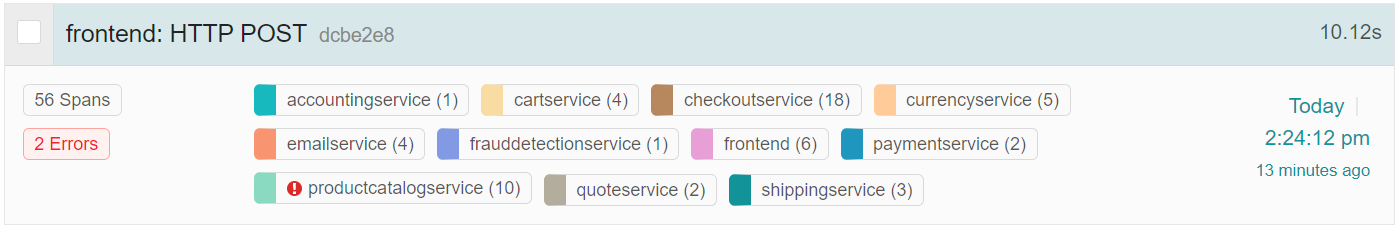
\includegraphics[width=15cm]{obrazky-figures/jeagerStopa.png}
  \caption{Stopa obsahující chybu}
  \label{fig:jeagerStopa}
\end{figure}

Na obrázku \ref{fig:jeagerStopa} vidíme stopu, ve které se vyskytují dvě chyby a vidíme červený vykřičník u~mikroslužby, kde nastaly chyby. Podrobnější informace se dozvíme po otevření detailu stopy.

\begin{listing}[H]
    \begin{minted}{json}
{
  "key": "otel.status_description",
  "type": "string",
  "value": 
      "_InactiveRpcError: <_InactiveRpcError of RPC that terminated with:
      tstatus = StatusCode.UNAVAILABLE
      tdetails = failed to connect to all addresses; 
      last error: UNKNOWN: ipv4:172.18.0.10:50053: 
      Failed to connect to remote host: Connection refused>"
}
\end{minted}
    \caption{Detailní informace o~chybě}
    \label{lst:jeagerError}
\end{listing}

Na výpisu \ref{lst:jeagerError} se nachází pole \texttt{status\textunderscore description}, jež je součástí detailu stopy v~monitorovacím nástroji Jeager. Vidíme, že mikroslužba na IP adrese 172.17.0.10 je nedostupná.


\subsection{Experiment č. 2: Přetížení aplikace v~důsledku mnoho aktivních uživatelů}

K~přetížení dochází, když aplikace zpracovává větší množství požadavků, než je schopna za danou dobu zpracovat. To může nastat z~několika důvodů například:
\begin{itemize}
    \item{velký počet aktivních uživatelů,}
    \item{aplikace zpracovává velký objem dat,}
    \item{aplikace není optimalizována pro svůj účel nebo zpracování dat.}
\end{itemize}
V~našem experimentu se budeme věnovat přetížení díky velkému počtu aktivních uživatelů.

\subsubsection{Navození nežádoucího stavu}

Přetížení nasimulujeme pomocí mikroslužby \texttt{load-generator}. V~základu simulujeme v~testovacím prostředí deset uživatelů a nyní zvýšíme počet na 500. 

\subsubsection{Výsledek}

Přetížení aplikace můžeme vypozorovat již v~úvodním grafu se stopami, kde si můžeme všimnout delší doby zpracování požadavků.

\begin{figure}[H]
  \centering
  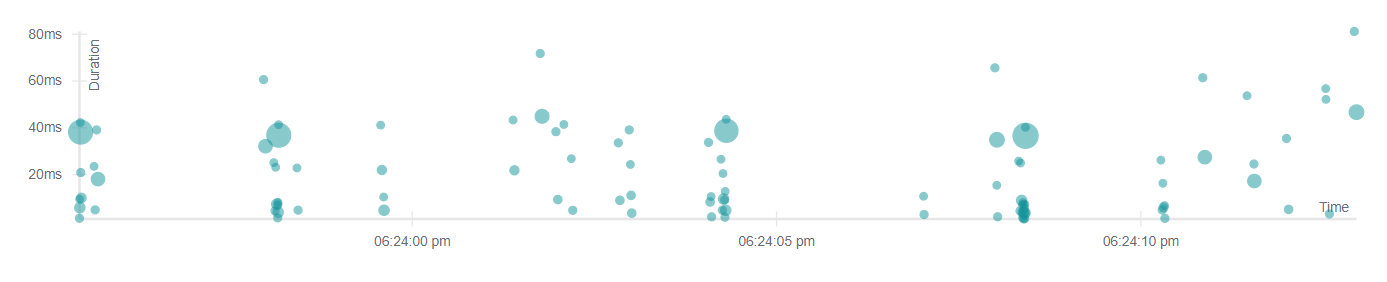
\includegraphics[width=15cm]{obrazky-figures/frontend-normal-graf.png}
  \caption{Úvodní graf délky požadavků u~uživatelského rozhraní}
  \label{fig:jeagerFrontendNormal}
\end{figure}

Na obrázku \ref{fig:jeagerFrontendNormal} vidíme požadavky mikroslužby \texttt{frontend}, která poskytuje uživatelské rozhraní. Můžeme vidět požadavky trvající maximálně 80 milisekund.


\begin{figure}[H]
  \centering
  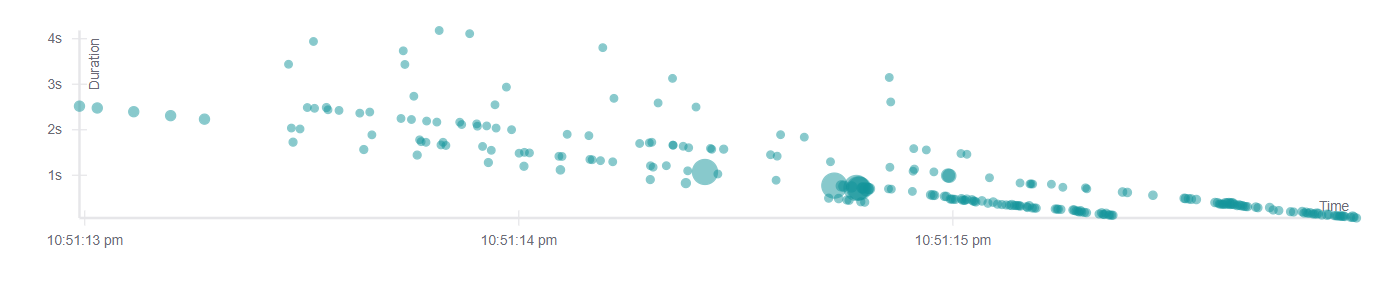
\includegraphics[width=15cm]{obrazky-figures/frontend_graf_users.png}
  \caption{Úvodní graf délky požadavků při přetížení}
  \label{fig:jeagerFrontendUsers}
\end{figure}

Na obrázku \ref{fig:jeagerFrontendUsers} vidíme, že délka požadavků se rapidně zvýšila. Požadavky nyní trvají až čtyři sekundy. Délka požadavku nemusí nutně znamenat přetížení aplikace. Proto se podíváme i na ostatní telemetrická data.


Pro přesnější diagnostikování problému se podíváme na metriky v~monitorovacím nástroji Grafana. 

\begin{figure}[H]
  \centering
  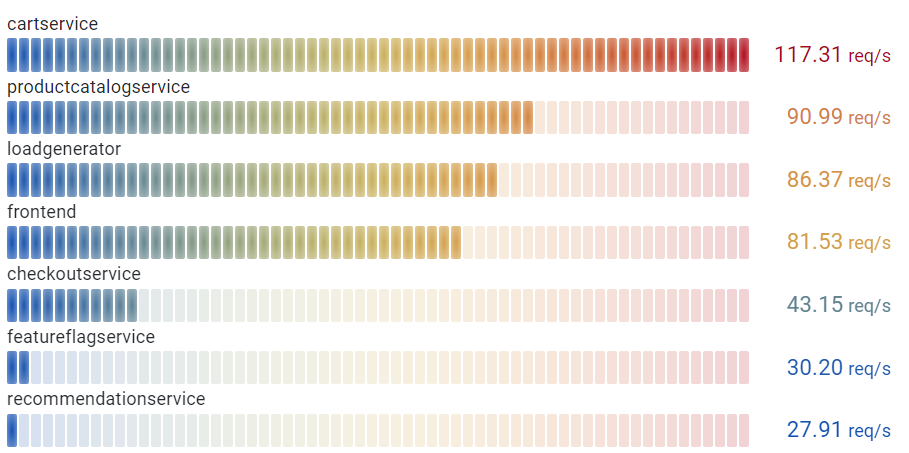
\includegraphics[width=13cm]{obrazky-figures/grafana_request.png}
  \caption{Graf s~požadavky na mikroslužby za sekundu}
  \label{fig:grafanaRequest}
\end{figure}

Na obrázku \ref{fig:grafanaRequest} vidíme počty požadavků za sekundu na sedm nejvytíženějších služeb testovací aplikace. Díky grafu vidíme, že služba \texttt{cartservice} je přetížená. Ostatním službám se také zvedl počet požadavků v~normálním poměru. V~důsledku toho můžeme určit, že se s~velkou pravděpodobností jedná o~přetížení aplikace z~důvodu velkého počtu aktivních uživatelů a nejedná se o~útok na aplikaci.

\begin{figure}[H]
  \centering
  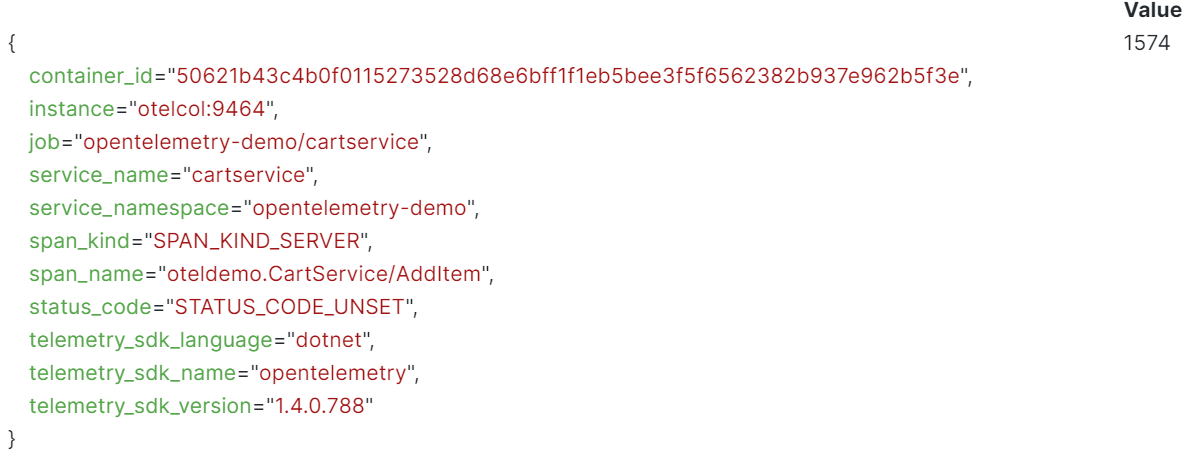
\includegraphics[width=13cm]{obrazky-figures/detail.png}
  \caption{Ukázka detailu počtu požadavku na koncový bod mikroslužby}
  \label{fig:grafanaRequestDetail}
\end{figure}

Na obrázku \ref{fig:grafanaRequestDetail} vidíme detailní popis metriky, která představuje počet požadavků na jeden koncový bod služby \texttt{cartservice}.
 

\subsection{Experiment č. 3: DoS útok na jednu z~mikroslužeb}

DoS (Denial of Service) je útok na počítačovou síť nebo webový server, při kterém útočník používá jeden počítač k~vytížení vybraného zdroje. Pokud by útočník používal více počítačů k~útoku jednalo by se o~distribuovaný útok DoS (DDoS).  Cílem je způsobit výpadek služby nebo její výrazné zpomalení cílového serveru. Hrozí zde ztráta dat, snížení odezvy dokonce výpadek celé služby.

\subsubsection{Navození nežádoucího stavu}

Útok nasimulujeme pomocí skriptu python, kde využijeme knihovnu \texttt{requests}\footnote{Dokumentace knihovny requests \url{https://pypi.org/project/requests/} [16.04.2023]} pro odeslání požadavku na testovací aplikaci. Odesílaní jednoho požadavku v~nekonečném cyklu by testovací aplikaci moc neohrozilo, proto využijeme také knihovnu \texttt{threading}\footnote{Dokumentace knihovny threading \url{https://docs.python.org/3/library/threading.html} [16.04.2023]}, díky které budeme odesílat požadavky ve více vláknech paralelně.

Nejprve se pomocí vývojářského okna v~prohlížeči v~záložce \textbf{Network} podíváme, jaké požadavky se v~testovací aplikaci nacházejí a jeden si vybereme.

\begin{figure}[H]
  \centering
  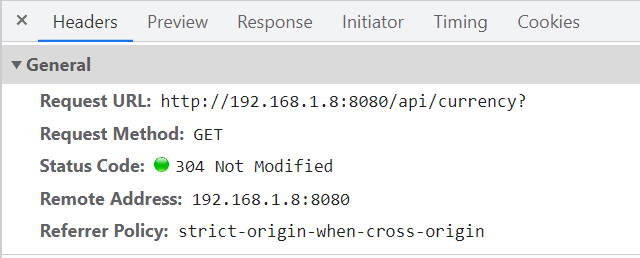
\includegraphics[width=10cm]{obrazky-figures/hlavicka.png}
  \caption{Hlavička požadavku z~prohlížeče}
  \label{fig:header}
\end{figure}

Na obrázku \ref{fig:header} vidíme hlavičku zachyceného požadavku v~prohlížeči, ze které vyčteme informace cílové adresy a o~jakou metodu HTTP se jedná.

\begin{listing}[H]
    \begin{minted}{python}
# Funkce k~provedení GET požadavku a výpisu odpovědi
def make_request():
    while True:
        response = requests.get("http://192.168.1.8:8080/api/currency")
        print(response.text)
\end{minted}
    \caption{Funkce pro odeslání požadavku GET}
    \label{lst:dos}
\end{listing}

Na výpisu \ref{lst:dos} vidíme vytvoření požadavku GET pomocí knihovny \texttt{requests} a výpisu odpovědi. Funkci zavoláme ve vytvořených vláknech a vlákna spustíme. Díku tomu docílíme nekonečného paralelního odesílání požadavků na testovací aplikaci.


\subsubsection{Výsledek}

Než si ukážeme, jaká telemetrická data se nám zobrazí, musíme si nejprve vysvětlit, jak mikroslužby mezi sebou komunikují, abychom později pochopili, jaké mikroslužby jsou přetížené. 

\begin{figure}[H]
  \centering
  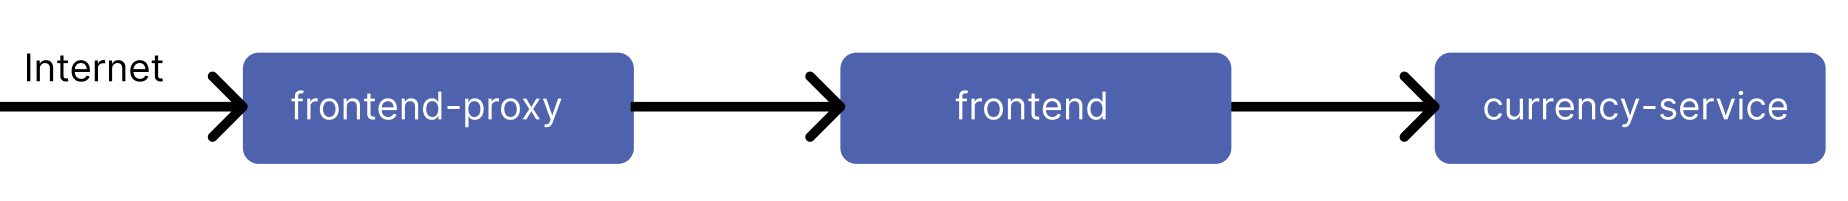
\includegraphics[width=15cm]{obrazky-figures/comunication.png}
  \caption{Komunikace mezi mikroslužbami}
  \label{fig:comunication}
\end{figure}

Na obrázku \ref{fig:comunication} vidíme, že uživatel nekomunikuje s~jednotlivými mikroslužbami přímo, ale komunikuje přes \texttt{frontend-proxy} a \texttt{frontend}. Pokud si tedy pro náš útok vybereme mikroslužbu \texttt{currency-service}, budou tím ovlivněny i předchozí dvě mikroslužby.

\begin{figure}[H]
  \centering
  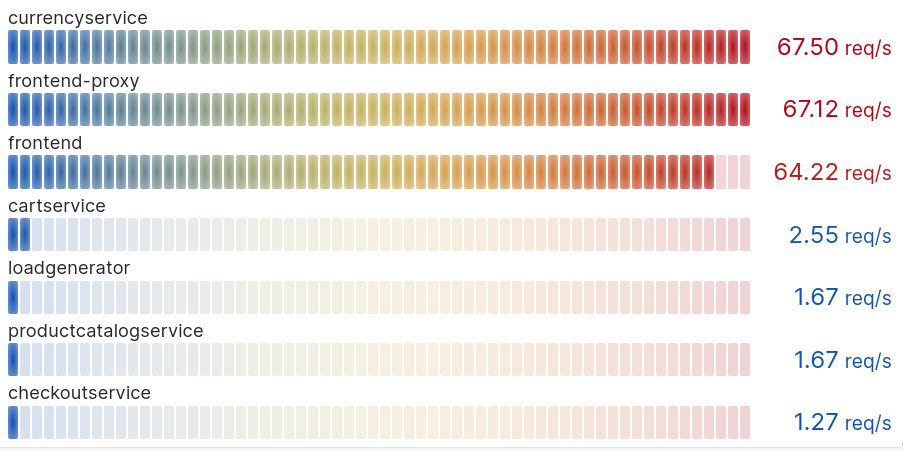
\includegraphics[width=13cm]{obrazky-figures/dos.png}
  \caption{Graf s~požadavky na mikroslužby za sekundu}
  \label{fig:dos}
\end{figure}

Na obrázku \ref{fig:dos} vidíme vysoké počty požadavků u~třech mikroslužeb, které jsou v~nepoměru s~ostatními službami. Z~toho můžeme usoudit, že nejspíš někdo odesílá velký počet požadavků na mikroslužbu \texttt{currencyservice} a aplikace se nachází pod DoS útokem. Pokud se chceme dozvědět více informací o~útočníkovi, musíme se podívat do detailu stopy.

\begin{figure}[H]
  \centering
  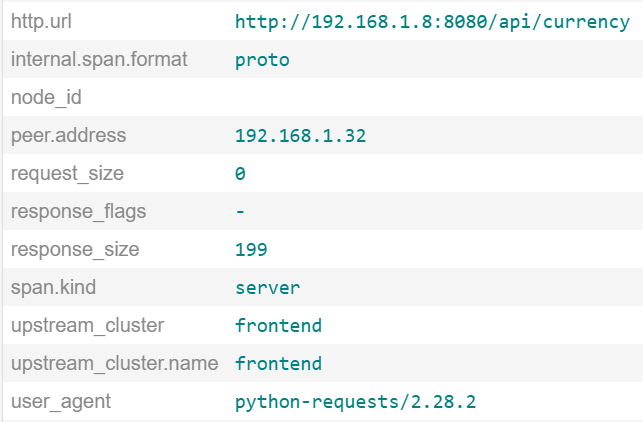
\includegraphics[width=12cm]{obrazky-figures/detailStopyJeager.png}
  \caption{Informace o~útočníkovi}
  \label{fig:detailDos}
\end{figure}

V~monitorovacím nástroji uvidíme velký počet stejných požadavků a po zobrazení detailu požadavku vidíme, že všechny pochází ze stejné adresy. Dozvídáme se i další informace jak vidíme na obrázku \ref{fig:detailDos} jako velikost požadavku a odpovědi, použitý nástroj pro odeslání požadavku atd.


\subsection{Experiment č. 4: Podvržení záznamu Syslog kolektoru}

Pomocí telemetrických dat můžeme automatizovat věci na serverech, jako například, vyvažování zátěže nebo nastavení upozornění, když přijde záznam, který bude obsahovat chybu, odešle se správci upozornění. Útočník by tím pádem mohl chtít telemetrická data podvrhnout, aby zmátl daný systém.

\subsubsection{Navození nežádoucího stavu}

Podvržený záznam Syslog budeme odesílat pomocí skriptu python. Záznamy Syslog se odesílají pomocí protokolu TCP nebo UDP. Pro získání portu, na kterém poslouchá kolektor záznamy Syslog, využijeme nástroj \texttt{nmap}. \texttt{Nmap} nám umožní detekovat otevřené porty na zadané IP adrese. Pokud se komunikace nachází na standardním portu, \texttt{nmap} nám řekne, že se jedná o~port pro komunikaci Syslog. Když se komunikace nachází na nestandardním portu, musíme využít nástroj \texttt{tcpdump} a zachytit na daných portech komunikaci. Pokud uživatel nepoužívá šifrovanou komunikaci, můžeme ze zachycených paketů přečíst záznam Syslog a zjistit, na jakém portu kolektor naslouchá záznamy.


\begin{listing}[H]
    \begin{minted}{python}
# Vytvoření TCP schránky
sock = socket.socket(socket.AF_INET, socket.SOCK_STREAM)
# Připojení ke vzdálenému TCP Syslog serveru
sock.connect(('192.168.1.14', 54527))
# Odesílání Syslog záznamu
sock.send(
    '<13>Apr 19 12:34:56 myhost myprocess: Hello, Syslog!\n'.encode())
# Uzavření schránka
sock.close()
\end{minted}
    \caption{Odeslání podvrženého záznamu na kolektor}
    \label{lst:SyslogZaznam}
\end{listing}

Na výpisu \ref{lst:SyslogZaznam} vidíme vytvoření schránky TCP a připojení na kolektor a odeslání podvrženého záznamu.

\subsubsection{Výsledek}

 \begin{figure}[H]
  \centering
  \includegraphics[width=15cm]{obrazky-figures/SyslogMes.png}
  \caption{Podvržený záznam v~monitorovacím nástroji}
  \label{fig:podvrh}
\end{figure}

Na obrázku \ref{fig:podvrh} vidíme záznam, jež jsme odeslali skriptem mezi ostatními záznamy ze Syslog serveru. 

Tomuto útoku můžeme lehce předejít. Syslog přijímač podporuje TSL protokol pro šifrování komunikace. Díky tomu si nikdo odchycené pakety nepřečte, ale ani nedokáže podvrhnout záznam.


\subsection{Zhodnocení experimentů}

Telemetrická data zobrazená v~monitorovacích nástrojích odpovídají prováděným experimentům a dali nám přesný pohled co se děje s~testovací aplikací. 


\chapter{Srovnání systému OpenTelemetry s~ostatními monitorovacími systémy}

V~této kapitole si ukážeme jiné nástroje pro sběr telemetrických dat a ukážeme si odeslání některých telemetrických dat od třetích stran do systému OpenTelemetry. Na konci kapitoly si porovnáme nástroje podle dat a architektury.


\section{Nástroj pro sběr záznamů Syslog}
\label{Syslog}

Syslog \cite{RFC3164} je standardizovaný protokol pro přenos záznamů po síti. Původně byl vyvinut pouze pro unixové operační systémy, ale nyní je podporován mnoha operačními systémy, síťovými zařízeními a aplikacemi. Protokol je navržen, aby poskytoval centralizovaný sběr, zpracování a uložení záznamů.


Systém OpenTelemetry umožňuje přijímat záznamy od protokolu Syslog. Podporuje jeho dva formáty záznamu RFC 3164 \cite{RFC3164} a RFC 5424 \cite{RFC5424}. Odesílání záznamů můžeme zajistit pomocí TCP nebo UDP protokolu. Využíváme rSyslog verze 8.2204.0.

\begin{figure}[H]
  \centering
  \includegraphics[width=13cm]{obrazky-figures/Syslog_topology.png}
  \caption{Schéma odesílání záznamů Syslog}
  \label{fig:SyslogTopology}
\end{figure}

Na obrázku \ref{fig:SyslogTopology} vidíme dva servery, kde běží operační systémy s~démonem Syslog, který přijímá systémové záznamy (kernel záznamy, mail záznamy, záznamy o~přihlášení atd.) a odesílá je na kolektor.

\begin{listing}[H]
    \begin{minted}{python}
*.*  action(type="omfwd"        # pomocí *.* odesíláme všechny záznamy
# Pokud je kolektor nedostupný, vytvoříme soubor s~neodeslanými 
# záznamy na disku, aby jsme o~ně nepřišly. Až je kolektor opět dostupný
# záznamy odešleme
queue.filename="fwdRule1"       # unikátní prefix pro soubor na disku
queue.maxdiskspace="1g"         # maximální velikost souboru
queue.saveonshutdown="on"       # uložení souboru při vypnutí
queue.type="LinkedList"         # asynchronní odesílání
action.resumeRetryCount="-1"    # počet pokusů při nedostupnosti kolektoru
                                # (-1 pro nekonečno)
# Nastavení adresu/doménu, port a protokol pro komunikaci s~kolektorem
Target="192.168.1.14" Port="54526" Protocol="tcp")
\end{minted}
    \caption{Konfigurace aplikace rSyslogu pro odesílání záznamů na kolektor}
    \label{lst:rSyslogConfig}
\end{listing}

Ve výpisu \ref{lst:rSyslogConfig} vidíme konfiguraci odesílání záznamů na vzdáleného hostitele (kolektor). Soubor s~konfigurací nalezneme v~\texttt{/etc/rSyslog.conf} nebo vytvoříme nový soubor s~příponou \texttt{*.conf} ve složce \texttt{/etc/rSyslog.d}. Využíváme k~tomu \texttt{omfwd}\footnote{Oficiální dokumentace omfwd modulu \url{https://www.rSyslog.com/files/temp/doc-indent/configuration/modules/omfwd.html} [14.03.2023]} modul, jež se nachází v~základním balíčku rSyslog, takže nemusí být dodatečně instalován a načítán. Můžeme specifikovat, jaké záznamy chceme odesílat.


Po odeslání záznamu musíme na kolektoru použít Syslog přijímač\footnote{Dokumentace Syslog přijímače \url{https://github.com/open-telemetry/opentelemetry-collector-contrib/tree/main/receiver/Syslogreceiver} [14.03.2023]}, který poskytuje systém OpenTelemetry. Přijímač přidáme v~konfiguračním souboru kolektoru, který využívá formát YAML\footnote{YAML Ain't Markup Language – formát pro serializaci dat textových souborů \url{https://yaml.org/} [14.03.2023]} pro ukládaní konfiguračních dat. Přijímač přidáme do položky \texttt{receivers}.


\begin{listing}[H]
    \begin{minted}{yaml}
receivers:
  Syslog/server:
    tcp:
      # přijímá záznamy ze všech IP adres na portu 54526
      listen_address: "0.0.0.0:54526"
    protocol: rfc5424
\end{minted}
    \caption{Konfigurace přijímače kolektoru pro příjem záznamů Syslog}
    \label{lst:rSyslogReciever}
\end{listing}

Ve výpisu \ref{lst:rSyslogReciever} vidíme nastavení přijímače pro příjem Syslog záznamů verze RFC 5424. Pro přenos záznamů využíváme TCP protokol a posloucháme na portu 54 526. Pro zobrazení využíváme monitorovací nástroj Loki od firmy Grafana, který pro filtrování záznamů vyžaduje štítek (label). Pro přidání štítku využijeme procesor kolektoru a každý záznam označíme štítkem.

\begin{listing}[H]
    \begin{minted}{yaml}
processors:
  attributes/server:
    actions:
      - action: insert
        key: Syslog
        value: server_eshop
      - action: insert
        key: loki.attribute.labels
        value: Syslog
\end{minted}
    \caption{Konfigurace procesoru kolektoru pro přidání štítku pro filtrování}
    \label{lst:SyslogProcesor}
\end{listing}

Ve výpisu \ref{lst:SyslogProcesor} vidíme vyžití atribut procesoru\footnote{Dokumentace atribut procesoru \url{https://github.com/open-telemetry/opentelemetry-collector-contrib/tree/main/processor/attributesprocessor} [14.03.2023]}, kde si prvně vytvoříme atribut s~jménem \texttt{Syslog} a hodnotou \texttt{server\textunderscore eshop} a poté z~něj vytvoříme atribut (štítek) pro monitorovací nastroj Loki. Po přijetí a přiřazení štítku můžeme daný záznam odeslat exportérem na monitorovací nástroj.

\begin{listing}[H]
    \begin{minted}{yaml}
exporters:
  loki:
    endpoint: "http://loki:3100/loki/api/v1/push"
\end{minted}
    \caption{Konfigurace exportéru kolektoru pro odeslání záznamu na monitorovací nástroj}
    \label{lst:SyslogExporter}
\end{listing}

Ve výpisu \ref{lst:SyslogExporter} vidíme exportér Loki\footnote{Dokumentace Loki exportéru \url{https://github.com/open-telemetry/opentelemetry-collector-contrib/tree/main/exporter/lokiexporter} [14.03.2023]}, který má definovaný koncový bod, kde monitorovací nástroj očekává záznamy.

\begin{figure}[H]
  \centering
  \includegraphics[width=15cm]{obrazky-figures/SyslogZaznam.png}
  \caption{Ukázka zobrazení záznamu}
  \label{fig:SyslogZaznam}
\end{figure}

Na obrázku \ref{fig:SyslogZaznam} vidíme Syslog záznam, kde celý záznam byl namapován automaticky na pole \texttt{body} struktury záznamu OpenTelemetry. Ze záznamu vyčteme, že se jedná o~varování pocházející z~docker démona o~selhání překladu adresy (resolver), který nedokázal číst z~DNS serveru.


\section{Analyzátor síťového provozu NetFlow}

NetFlow \cite{RFC3954} je síťový protokol, který sbírá a analyzuje data o~provozu IP. Správcům sítě poskytuje přehled o~síťovém provozu a pomáhá při analýze chování sítě, což pomáhá při optimalizaci výkonu sítě, identifikaci bezpečnostních hrozeb atd.

NetFlow funguje na principu zaznamenávaní síťových toků. Tok je definován jako posloupnost paketů, které mají společnou charakteristiku, jakou jsou stejné zdrojové a cílové IP adresy, čísla portů, protokol a hodnotu priority komunikace (ToS). Tok obsahuje informace také o~velikosti přenesených dat, počtu paketů, počáteční a koncový čas toku atd.

Zachytíme toky v~síti testovací aplikace pomocí protokolu NetFlow a podíváme se, jaké informace nám poskytnou.

\begin{figure}[H]
  \centering
  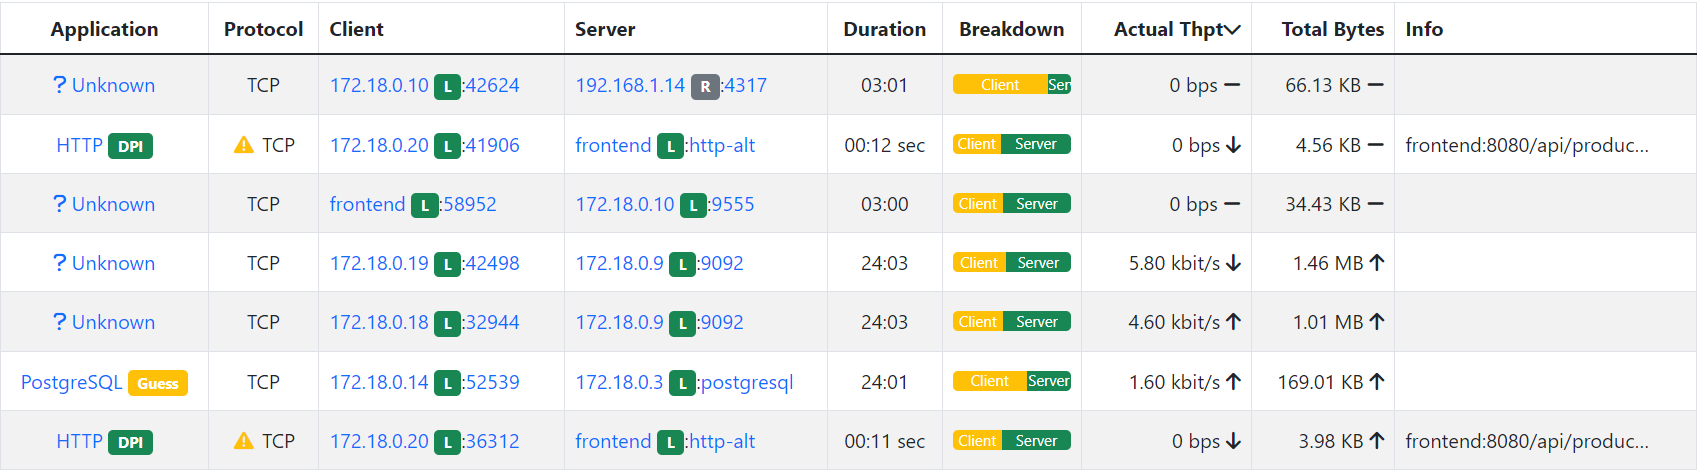
\includegraphics[width=15cm]{obrazky-figures/flows.png}
  \caption{Ukázka toků z~nástroje ntopng}
  \label{fig:flow}
\end{figure}

Na obrázku \ref{fig:flow} vidíme aktuální toky. Můžeme vidět, že NetFlow protokol nám neposkytuje detailní informace o~mikroslužbách a zpracování jejich požadavků jako telemetrická data systému OpenTelemtry. Poskytuje nám přehled o~síťové komunikaci mezi jednotlivými mikroslužbami nebo komunikaci s~kolektorem systému OpenTelemetry.

\section{Nástroj pro monitorovaní a správu sítě SNMP}
 SNMP \cite{RFC1157} neboli Simple Network Management Protocol je standardizovaný internetový protokol, jenž poskytuje správci sítě správu a monitorování síťových zařízení, jako jsou například směrovače, přepínače, servery a další. Umožňuje správcům sítě spravovat a monitorovat zařízení z~jednoho místa. Poskytuje informace o~výkonu sítě, využití šířky pásma, ale můžeme sledovat informace i o~stavu a konfiguraci jednotlivých síťových zařízení, jako je využití paměti, zatížení CPU nebo verzi bežícího firmwaru.

 SNMP funguje na principu manager-agent, kde stanice správce vystupuje jako manager a jednotlivá síťová zařízení jako agenti. Manager odesílá požadavky na agenty, aby získal informace o~stavu zařízení.

 Data v~SNMP jsou reprezentována pomocí Management Information Base (MIB). MIB je databáze obsahující hierarchicky organizované informace o~spravovaných zařízeních a sítích. Každý objekt je identifikován pomocí jedinečného čísla (OID). OID se skládá z~řady čísel, které jsou odděleny tečkou. Například OID může vypadat takto: 1.3.6.1.1.2.1.

 \begin{figure}[H]
  \centering
  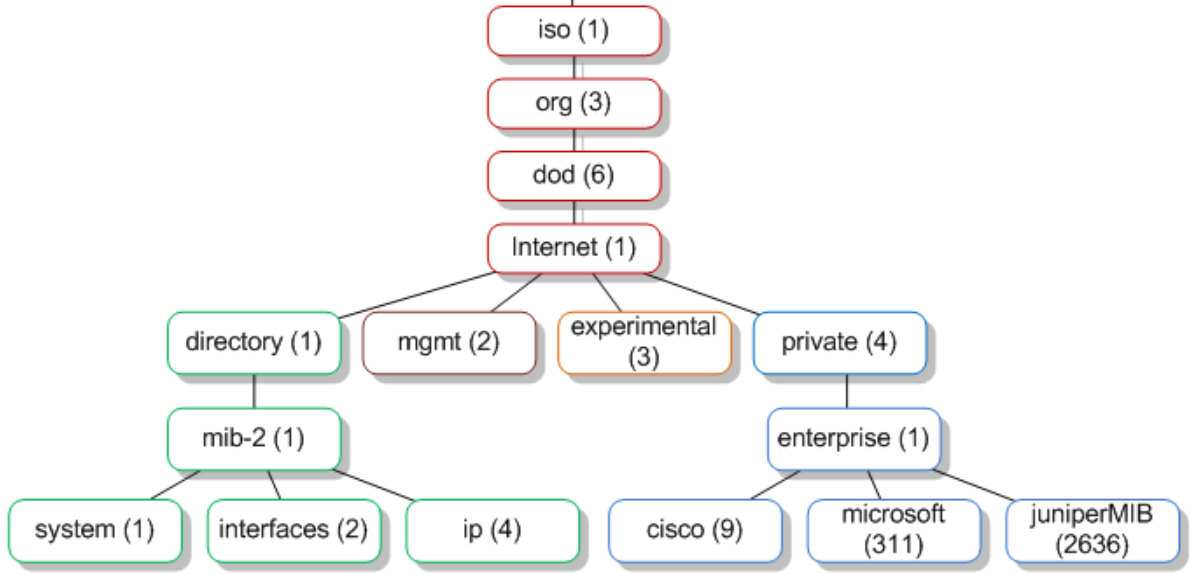
\includegraphics[width=15cm]{obrazky-figures/mib.png}
  \caption{OID stromová struktura}
  \label{fig:mib}
\end{figure}

Na obrázku \ref{fig:mib} vidíme stromovou strukturu OID. Uzel \texttt{system} je reprezentován již zmíněným identifikátorem z~ukázky 1.3.6.1.1.2.1.

Ukážeme si, jaká data nám může zobrazit SNMP o~testovací aplikaci. Data budeme číst z~prvku OID 1.3.6.1.2.1.25.4.2 neboli \texttt{hrSWRunEntry}.

\begin{table}[H]
\centering
\begin{tabular}{|p{3.5cm}|p{3.4cm}|p{5.8cm}|}
\hline
\textbf{Název} & \textbf{OID} & \textbf{Popis} \\ \hline
hrSWRunIndex & 1.3.6.1.2.1.25.4.2.1.1 & Unikátní hodnota programového vybavení \\ \hline
hrSWRunName & 1.3.6.1.2.1.25.4.2.1.2 & Název programového vybavení \\ \hline
hrSWRunID & 1.3.6.1.2.1.25.4.2.1.3 & ID produktu běžícího programu\\ \hline
hrSWRunPath & 1.3.6.1.2.1.25.4.2.1.4 & Umístění na disku hostitele\\ \hline
hrSWRunParameters & 1.3.6.1.2.1.25.4.2.1.5 & Parametry, které byly dodány při prvním načtení\\ \hline
hrSWRunType & 1.3.6.1.2.1.25.4.2.1.6 & Typ programu: 'unknown': 1, 'operatingSystem': 2, 'deviceDriver': 3, 'application': 4. \\ \hline
hrSWRunStatus & 1.3.6.1.2.1.25.4.2.1.7 & Status o~běhu programu: 'running': 1, 'runnable': 2, 'notRunnable': 3, 'invalid': 4. \\ \hline
\end{tabular}
\caption{Potomky prvku hrSWRunEntry}
\end{table}

Pro čtení SNMP dat využijeme nástroj snmpwalk\footnote{Manuál nástroje snmpwalk \url{https://linux.die.net/man/1/snmpwalk} [16.04.2023]}. Nejprve si vypíšeme názvy programového vybavení hostitele a podíváme se na programy související s~testovací aplikací.

\begin{listing}[H]
    \begin{minted}{bash}
snmpwalk -v2c -c public localhost 1.3.6.1.2.1.25.4.2.1.2
\end{minted}
    \caption{Výpis hrSWRunName pomocí nástroje snmpwalk}
    \label{lst:snmpwalk}
\end{listing}

Pomocí příkazu ve výpisu \ref{lst:snmpwalk} si vypíšeme všechny názvy programového vybavení na hostiteli. Jelikož výsledek je velmi dlouhý, ukážeme si jen část, kde se budou nacházet položky, tykající se testovací aplikace.

\begin{listing}[H]
    \begin{minted}{bash}
iso.3.6.1.2.1.25.4.2.1.2.2931 = STRING: "docker-proxy"
iso.3.6.1.2.1.25.4.2.1.2.2985 = STRING: "shippingservice"
iso.3.6.1.2.1.25.4.2.1.2.3813 = STRING: "locust"
iso.3.6.1.2.1.25.4.2.1.2.3820 = STRING: "productcatalogs"
\end{minted}
    \caption{Část výsledku příkazu pro výpis hrSWRunName}
    \label{lst:snmpwalkResult}
\end{listing}

Na výpisu \ref{lst:snmpwalkResult} vidíme \texttt{docker-proxy}, které je zodpovědné za probíhající komunikaci mezi kontejnery a hostitelem. Dále vidíme tři mikroslužby. V~následujících tabulkách si ukážeme informace, které nám SNMP poskytne o~jedné mikroslužbě a docker-proxy. Na jednotlivé informace se budeme dotazovat na konkrétní programové vybavení a to docílíme tím, když OID rozšíříme o~poslední číslo z~výsledku. Například pro dotazování na docker-proxy pro zjištění hrSWRunIndex použijeme OID 1.3.6.1.2.1.25.4.2.1.1.2931.


\begin{table}[H]
\centering
\begin{tabular}{|p{3.5cm}|p{6cm}|p{3.8cm}|}
\hline
 & \textbf{docker-proxy} & \textbf{shippingservice} \\ \hline
hrSWRunIndex & 2931 & 2985 \\ \hline
hrSWRunName & docker-proxy & shippingservice \\ \hline
hrSWRunID & ccitt.0 & ccitt.0\\ \hline
hrSWRunPath & /usr/bin/docker-proxy & /app/shippingservice\\ \hline
hrSWRunParameters & -proto tcp -host-ip :: -host-port 9001 -container-ip 172.18.0.6 -container-port 9001 & \\ \hline
hrSWRunType & 4 & 4 \\ \hline
hrSWRunStatus & 2 & 2\\ \hline
\end{tabular}
\caption{Informace ze SNMP}
\label{tbl:info}
\end{table}

Z~tabulky \ref{tbl:info} vidíme, že se dozvídáme pouze informace o~kontejneru, jako je IP adresa a port a název mikroslužby, a zda běží. SNMP nám neříká žádné informace o~mikroslužbě samotné jako například její vytížení, odezvu, komunikaci atd.

\section{Srovnání jiných nástrojů se systémem OpenTelemetry}

V~této podkapitole si srovnáme zmíněné nástroje se systémem OpenTelemetry a porovnáme je podle architektury a zda by nám byly schopny ukázat nežádoucí stavy z~experimentů.

\subsection{Srovnání podle architektury}

Architekturu systému OpenTelemetry jsme si popsali ve druhé kapitole \ref{architektura}, tak si ukážeme pouze architekturu nástrojů zmíněných v~této kapitole.

\subsubsection{Architektura Syslog}
Démon Syslog běží na pozadí a přijímá záznamy. Může přijímat záznamy od procesu, služby nebo aplikace bežící na počítači, která generuje záznamy o~svém běhu. Záznamy ukládá v~textových souborech nebo odesílá na server Syslog.

\subsubsection{Architektura NetFlow}
Architektura se skládá ze tří prvků exportér, kolektor a analyzátor. Exportér vložíme do síťové komunikace jako nezávislou sondu, která bude poslouchat komunikaci, vytvářet toky a odesílat je na kolektor. Kolektor ukládá jednotlivé toky pro analyzátor. Pomocí analyzátoru studujeme jednotlivé toky a získáváme z~nich užitečné informace.

\subsubsection{Architektura SNMP}
Architektura SNMP obsahuje dva prvky manažera a agenty. Agent představuje monitorovaný prvek a manažer je stanice, která odesílá požadavky na agenty a získává data.


\subsection{Srovnání podle dat}
Porovnáme zmíněné nástroje, zda by nám byly schopny detekovat nežádoucí stavy navozené experimenty.

\subsubsection{Nástroj Syslog}
Syslog by nám nebyl schopný detekovat ani jeden z~experimentů, jelikož v~našem testovacím prostředí nevidí do mikroslužeb. Jediný experiment, který by jsme mohli odhalit, je podvržení záznamu Syslog. Kdyby správce porovnal záznamy uložené na serveru se záznamy v~monitorovacím nástroji, mohl by si všimnout, že v~monitorovacím nástroji se nachází záznamy, které nejsou uloženy na serveru.

\subsubsection{Analyzátor NetFlow}
NetFlow nám umožní lehce detekovat dva experimenty a to přetížení pomocí mnoho aktivních uživatelů a DoS útok. Uvidíme veliké množství nových toků. Experimenty rozlišíme od sebe pomocí zdrojové IP adresy v~toku, kde DoS útok bude mít všude stejnou adresu a přetížení bude obsahovat rozdílné adresy. Výpadek a podvržení poznáme trochu obtížněji. Musíme pozorovat toky a mít znalost, které toky se běžně objevují. U~podvrženého záznamu uvidíme tok, který obsahuje cílovou adresu kolektoru systému OpenTelemetry a zdrojová adresa nebude serveru, kde běží testovací aplikace. Výpadek mikroslužby poznáme, že toky se přestanou objevovat.

\subsubsection{Nástroj SNMP}
Nástroj SNMP nám pomůže při detekci prvních třech experimentů. Protože nám poskytuje informaci akorát o~tom zda mikroslužba běží nebo ne. Nepoznáme, ale z~jakého důvodu mikroslužba neběží.


\subsection{Závěrečné srovnání}

Vidíme, že představené nástroje v~kapitole pět nám nedávají moc přehled o~dění v~mikroslužbách a nemůžeme pomocí nich většinou detekovat jejich chování, ale je to i dáno jejich architekturou, protože jediný systém OpenTelemetry běží uvnitř mikroslužby a tak je nám schopný poskytovat informace o~vnitřním chodu.


\chapter{Závěr}

Cílem práce bylo prozkoumat nový systém OpenTelemetry, jež má sloužit jako jednotný nástroj pro sběr telemetrických dat. Nástroj je zaměřen na sběr dat z~cloudových aplikací. Proto nemůžeme říct, že budeme využít pouze systém OpenTelemetry pro monitorování celé infrastruktury. Jedná se spíše o~komplement k~zmíněným nástrojům, protože například o~strojích, na kterých aplikace běží by nám poskytl minimální informace.

Ze začátku práce jsem musel nastudovat, co je systém OpenTelemetry a jak funguje. Pro testovací prostředí jsem si vybral demo aplikaci, kterou poskytují samotní tvůrci. Prostředí jsem rozdělil na dvě části, aby mohly běžet nezávisle na dvou serverech. Jedná část obsahuje webový obchod a druhá část je kolektor s~monitorovacími nástroji. Dále jsem vložil do testovacího prostředí jiné nástroje a pozoroval jaké data nám poskytnout. Poté jsem prováděl experimenty nad prostředím a pozoroval jsem, zda budou telemetrická data odpovídat danému nežádoucímu stavu.


Jedná se o~nový standard, který se stále vyvíjí. V~průběhu práce se stalo, že se třikrát změnila konfigurace jednoho z~procesorů v~kolektoru a chybí podpora generování některých telemetrických dat u~určitých technologií, převážně se jedná o~záznamy. Přesto tento nástroj hodnotím velmi kladně. Jako jediný nástroj ze zmíněných v~práci, nám poskytl přehled o~vnitřním chodu mikroslužeb. Díky němu můžeme vidět počty požadavků na jednotlivé koncové body mikroslužeb, jejich odezvy, přerušení spojení mezi mikroslužbami. Poskytuje nám i detailní informace o~jednotlivých požadavcích. Z požadavku můžeme udělat stopu, jež se skládá z více operacích, pomocí automatického generování telemetrických dat. Pokud nám nestačí automatické rozdělení požadavku, můžeme ho manuálně rozdělit na operace a podívat se, která část tvrdá nejdéle a jaké informace obsahují.

S největším problémem v této bakalářské práci jsem se setkal u čtení dat z paketu. Nemohl jsem najít správné soubory .proto, pomocí kterých převádíme serializovaná binární data na čitelná pro člověka.

Největší přínos tato bakalářská práce poskytne lidem, kteří se rozhodují využít systému OpenTelemetry. Poskytne jim informace jak generovat telemetrická data z~aplikace, jak je sbírat a zobrazovat v~monitorovacím nástroji.


